% Rapport AmanaBank — Overleaf (fichier unique)
% Compiler avec pdfLaTeX — images dans images/
\documentclass[11pt,a4paper,twoside,openright]{report}

% ── Encodage & langue ──────────────────────────────────────────────
\usepackage[T1]{fontenc}
\usepackage[utf8]{inputenc}
\usepackage[french]{babel}

% ── Typographie (Palatino moderne) ─────────────────────────────────
\usepackage{newpxtext,newpxmath}
\usepackage[scaled=0.92]{helvet}
\usepackage{courier}
\renewcommand{\familydefault}{\rmdefault}
\usepackage{microtype}

% ── Mise en page ───────────────────────────────────────────────────
\usepackage{geometry}
\geometry{left=2.8cm, right=2.5cm, top=2.8cm, bottom=2.8cm, headheight=15pt}
\usepackage{setspace}
\onehalfspacing

% ── Couleurs AmanaBank ─────────────────────────────────────────────
\usepackage[table]{xcolor}
\definecolor{AmanaBrown}{HTML}{4B3621}
\definecolor{AmanaBrownMid}{HTML}{6B5344}
\definecolor{AmanaGold}{HTML}{A6893A}
\definecolor{AmanaGoldLight}{HTML}{C9A84C}
\definecolor{AmanaBeige}{HTML}{F9F6F1}
\definecolor{AmanaBeigeDark}{HTML}{EDE6DA}
\definecolor{AmanaText}{HTML}{3A2E22}

% ── Graphiques & tableaux ──────────────────────────────────────────
\usepackage{graphicx}
\usepackage{float}
\usepackage{booktabs}
\usepackage{longtable}
\usepackage{array}
\usepackage{multirow}
\usepackage{tabularx}
\usepackage{colortbl}
\usepackage{etoolbox}
\usepackage{caption}

\captionsetup{
    font=small,
    labelfont={bf,color=AmanaBrown},
    textfont=color=AmanaText,
    skip=8pt
}

\AtBeginEnvironment{tabular}{\renewcommand{\arraystretch}{1.28}}
\AtBeginEnvironment{tabularx}{\renewcommand{\arraystretch}{1.28}}
\BeforeBeginEnvironment{table}{\rowcolors{2}{AmanaBeige!40}{white}}

\newcommand{\tabhead}[1]{\textcolor{white}{\textbf{#1}}}
\newcolumntype{L}{>{\raggedright\arraybackslash}X}
\newcolumntype{C}{>{\centering\arraybackslash}X}

% ── Liens & code ───────────────────────────────────────────────────
\usepackage{hyperref}
\hypersetup{
    colorlinks=true,
    linkcolor=AmanaBrown,
    citecolor=AmanaBrownMid,
    urlcolor=AmanaGold,
    pdfborder={0 0 0}
}
\usepackage{listings}
\usepackage{amsmath}
\usepackage{enumitem}
\setlist[itemize]{leftmargin=*, itemsep=0.25em}
\setlist[enumerate]{leftmargin=*, itemsep=0.25em}

\lstset{
    basicstyle=\ttfamily\small,
    breaklines=true,
    frame=single,
    rulecolor=\color{AmanaBeigeDark},
    backgroundcolor=\color{AmanaBeige},
    keywordstyle=\color{AmanaBrown}\bfseries,
    commentstyle=\color{AmanaBrownMid},
    stringstyle=\color{AmanaGold}
}

% ── Titres & en-têtes ──────────────────────────────────────────────
\usepackage{titlesec}
\usepackage{tikz}
\usetikzlibrary{calc}
\usepackage{fancyhdr}
\usepackage{tocloft}

\renewcommand{\thechapter}{\arabic{chapter}}
\renewcommand{\chaptername}{Chapitre}

\titleformat{\chapter}[display]
  {\normalfont\huge\bfseries\color{AmanaBrown}}
  {\chaptertitlename\ \thechapter}
  {14pt}
  {\Huge}
  [\vspace{0.4em}{\color{AmanaGold}\titlerule[1.2pt]}\vspace{0.6em}]

\titlespacing*{\chapter}{0pt}{-8pt}{28pt}

\titleformat{\section}
  {\normalfont\Large\bfseries\color{AmanaBrown}}{\thesection}{0.8em}{}
\titleformat{\subsection}
  {\normalfont\large\bfseries\color{AmanaBrownMid}}{\thesubsection}{0.8em}{}

\pagestyle{fancy}
\fancyhf{}
\fancyhead[L]{\small\color{AmanaBrownMid}\leftmark}
\fancyhead[R]{\small\color{AmanaBrownMid}\thepage}
\renewcommand{\headrule}{\color{AmanaGold}\hrule width\headwidth height 0.6pt}
\fancyfoot[C]{}

\fancypagestyle{plain}{
  \fancyhf{}
  \fancyfoot[C]{\small\color{AmanaBrownMid}\thepage}
  \renewcommand{\headrulewidth}{0pt}
}

\graphicspath{{images/}}

\newcommand{\includefigure}[5]{%
  \begin{figure}[H]
    \centering
    \IfFileExists{#1}{%
      \includegraphics[#2]{#3}%
    }{%
      \fbox{\parbox{0.9\textwidth}{\centering\vspace{1.5cm}
      \textit{\color{AmanaBrownMid}[#4 — fichier attendu : \texttt{#1}]}
      \vspace{1.5cm}}}%
    }
    \caption{#4}
    \label{#5}
  \end{figure}%
}

% ── Informations du projet ───────────────────────────────────────────
\newcommand{\anneeuniv}{2025/2026}
\newcommand{\etudianteun}{BENSOUDA Amina}
\newcommand{\etudiantedeux}{AFILAL Soraya}
\newcommand{\encadrante}{Dr. ORCHI HOUDA}
\newcommand{\ecole}{École Marocaine des Sciences de l'Ingénieur}
\newcommand{\villeecole}{de Rabat}
\newcommand{\filiere}{Ingénierie Informatique et Réseaux}
\newcommand{\niveau}{3\textsuperscript{e} année}
\newcommand{\titreprojet}{Système de gestion d'agence bancaire}
\newcommand{\nomapplication}{AmanaBank}
\newcommand{\organisme}{École Marocaine des Sciences de l'Ingénieur — Rabat}

\begin{document}

\pagenumbering{roman}
\thispagestyle{empty}
\begin{titlepage}
\begin{tikzpicture}[remember picture, overlay]
  \fill[AmanaBrown] (current page.north west) rectangle ([yshift=-3.2cm]current page.north east);
  \fill[AmanaBeige] (current page.south west) rectangle ([yshift=6.2cm]current page.south east);
  \draw[AmanaGold, line width=1.4pt]
    ([yshift=-3.2cm]current page.north west) -- ([yshift=-3.2cm]current page.north east);
  \draw[AmanaGold, line width=1.4pt]
    ([yshift=6.2cm]current page.south west) -- ([yshift=6.2cm]current page.south east);
\end{tikzpicture}

\begin{center}
\vspace*{0.35cm}
{\color{white}\large\bfseries Année universitaire \anneeuniv}\\[0.25cm]
{\color{AmanaGoldLight}\normalsize \ecole{} --- Rabat}

\vspace{1.6cm}

\IfFileExists{images/amana-logo.png}{%
  
\includegraphics[width=0.34\textwidth]{amana-logo.png}%
}{%
  {\color{AmanaBrown}\Huge\bfseries \nomapplication}%
}\\[1.4cm]

{\color{AmanaBrown}\LARGE\bfseries Rapport de Projet de Fin d'Année}\\[0.45cm]
{\color{AmanaText}\large \niveau\ --- \filiere}\\[1.6cm]

{\color{AmanaGold}\large\textsc{Sous le thème de}}\\[0.45cm]
{\color{AmanaBrown}\huge\bfseries \titreprojet}\\[0.35cm]
{\color{AmanaBrown}\Large Application web \textbf{\nomapplication}}

\vfill

\begin{minipage}{0.82\textwidth}
\centering
\arrayrulecolor{AmanaGold}
\begin{tabular}{@{}>{\columncolor{AmanaBeige}}p{0.82\textwidth}@{}}
\\[-0.5em]
\centering
\textbf{\large\color{AmanaBrown} Réalisé par}\\[0.55em]
{\large\color{AmanaText} \etudianteun}\\[0.15em]
{\large\color{AmanaText} \etudiantedeux}\\[1.1em]
\textbf{\large\color{AmanaBrown} Encadrée par}\\[0.4em]
{\large\color{AmanaText} \encadrante}\\[1.1em]
{\large\color{AmanaText} \ecole}\\[0.1em]
{\large\color{AmanaText} \villeecole}
\end{tabular}
\end{minipage}

\vspace{1.4cm}
\end{center}
\end{titlepage}

\chapter*{Dédicaces}
\addcontentsline{toc}{chapter}{Dédicaces}

Nous dédions ce projet de fin d'année à nos parents, dont le soutien inébranlable, l'amour et les encouragements constants ont été des piliers essentiels tout au long de notre parcours académique. Leur confiance en nos capacités nous a toujours inspirées à donner le meilleur de nous-mêmes.

À \encadrante, notre encadrante, pour ses conseils avisés, sa disponibilité et son expertise. Merci pour votre soutien inestimable et votre guidance précieuse tout au long de ce projet.

Nous souhaitons également exprimer notre profonde gratitude envers l'ensemble du corps professoral de l'\ecole\ pour la qualité de la formation reçue et l'exigence qui nous a permis de développer des compétences techniques et une rigueur professionnelle.

Enfin, nous dédions ce travail à toutes les personnes qui, de près ou de loin, ont contribué à notre développement personnel et académique.

\chapter*{Remerciements}
\addcontentsline{toc}{chapter}{Remerciements}

Nous tenons tout d'abord à remercier chaleureusement \encadrante, pour sa guidance experte, son soutien constant et ses précieux conseils tout au long de ce projet. Son expertise et son enthousiasme ont été une source d'inspiration et ont grandement enrichi notre expérience académique.

Nous remercions cordialement tout le corps professoral et administratif de l'\ecole\ pour son accompagnement tout au long de notre formation en \filiere.

Nous sommes reconnaissantes envers nos familles et nos proches pour leur soutien inconditionnel et leur compréhension durant cette période intensive. Leur encouragement a été le moteur de notre persévérance.

Enfin, merci à toutes les personnes qui ont participé, de près ou de loin, à l'élaboration de ce projet.

\vspace{1cm}
\begin{flushright}
    À toutes et à tous… merci.
\end{flushright}

\chapter*{Résumé}
\addcontentsline{toc}{chapter}{Résumé}

La gestion quotidienne d'une agence bancaire implique le traitement de données clients sensibles, la tenue rigoureuse des comptes et l'exécution d'opérations financières soumises à des règles métier strictes. Les méthodes traditionnelles, souvent manuelles ou dispersées, augmentent les risques d'erreurs de saisie, d'incohérences de solde et de faible traçabilité.

Face à ces limites, ce projet propose \textbf{\nomapplication}, une application web centralisée développée avec \textbf{Java} et \textbf{Spring Boot} par \etudianteun\ et \etudiantedeux\ dans le cadre d'un projet de fin d'année à l'\ecole.

La solution couvre la gestion interne de l'agence (clients, comptes, transactions, utilisateurs, audit, reporting) ainsi que des extensions : paiement de factures, commande de chéquier, centre de notifications et portail client en ligne. Chaque acteur dispose d'un espace adapté à son rôle.

Le présent rapport présente le contexte du projet, l'analyse des besoins, la conception UML, l'environnement technique, l'architecture logicielle, la réalisation des interfaces et les perspectives d'évolution.

\vspace{0.5cm}
\textbf{Mots-clés :} Agence bancaire — Spring Boot — Gestion de comptes — Transactions — Portail client — UML

\chapter*{Abstract}
\addcontentsline{toc}{chapter}{Abstract}

Daily operations in a bank branch involve sensitive customer data, strict account management, and financial transactions governed by business rules. Traditional, often manual approaches increase the risk of data entry errors, balance inconsistencies, and poor traceability.

To address these challenges, this project introduces \textbf{\nomapplication}, a centralized web application built with \textbf{Java} and \textbf{Spring Boot} by \etudianteun\ and \etudiantedeux\ as part of a final-year project at EMSI Rabat.

The solution supports internal branch management (clients, accounts, transactions, users, audit, reporting) as well as extended features: bill payments, checkbook orders, an in-app notification center, and an online client portal. Each stakeholder has a role-based workspace.

This report presents the project context, requirements analysis, UML design, technical environment, software architecture, interface implementation, and future perspectives.

\vspace{0.5cm}
\textbf{Keywords:} Bank branch — Spring Boot — Account management — Transactions — Client portal — UML

\tableofcontents
\clearpage
\listoffigures
\clearpage
\listoftables
\clearpage
\chapter*{Liste des abréviations}
\addcontentsline{toc}{chapter}{Liste des abréviations}

\begin{tabular}{@{}ll@{}}
    \rowcolors{2}{AmanaBeige!40}{white}
    \toprule
    \rowcolor{AmanaBrown}\color{white}
    \textbf{Abréviation} & \textbf{Signification} \\
    \midrule\color{AmanaText}
    API     & Application Programming Interface \\
    BCrypt  & Algorithme de hachage de mots de passe \\
    CRUD    & Create, Read, Update, Delete \\
    CSS     & Cascading Style Sheets \\
    HTML    & HyperText Markup Language \\
    HTTP    & Hypertext Transfer Protocol \\
    JPA     & Java Persistence API \\
    JWT     & JSON Web Token \\
    KPI     & Key Performance Indicator \\
    MCD     & Modèle Conceptuel de Données \\
    MLD     & Modèle Logique de Données \\
    MVC     & Model-View-Controller \\
    ORM     & Object-Relational Mapping \\
    PDF     & Portable Document Format \\
    PFA     & Projet de Fin d'Année \\
    SQL     & Structured Query Language \\
    UML     & Unified Modeling Language \\
    \bottomrule
\end{tabular}

\clearpage

\pagenumbering{arabic}
\setcounter{page}{1}

\chapter*{Introduction générale}
\addcontentsline{toc}{chapter}{Introduction générale}
\label{ch:intro}

\section{Contexte général}

La digitalisation des services bancaires constitue aujourd'hui un enjeu majeur pour les établissements financiers. Au sein d'une agence, les agents traitent quotidiennement des demandes variées : ouverture de comptes, dépôts, retraits, virements, consultation d'historiques et supervision des opérations. Sans outil centralisé, ces tâches reposent souvent sur des registres papier, des fichiers tableur ou des logiciels non intégrés, ce qui complique le contrôle des soldes et la traçabilité des actions.

Dans le cadre de notre formation en \filiere\ à l'\ecole, nous avons développé \textbf{\nomapplication}, un système web de gestion d'agence bancaire répondant au cahier des charges du projet de fin d'année (PFA). Ce travail s'inscrit dans une démarche de conception rigoureuse (UML, modèle de données) suivie d'une implémentation incrémentale en Java.

\section{Problématique}

Comment concevoir et réaliser une application web fiable permettant à une agence bancaire de :
\begin{itemize}[leftmargin=*]
    \item centraliser la gestion des clients et de leurs comptes ;
    \item exécuter des opérations financières en respectant les règles métier (solde, statut des comptes) ;
    \item assurer la traçabilité des actions sensibles et la sécurité des accès ;
    \item offrir au client un espace de consultation et de suivi en ligne ?
\end{itemize}

Les approches manuelles ne garantissent ni la cohérence des soldes, ni l'identification de l'agent exécutant, ni une supervision efficace pour le chef d'agence.

\section{Objectifs du projet}

Les objectifs principaux sont :
\begin{enumerate}[leftmargin=*]
    \item \textbf{Analyser} le besoin à partir du cahier des charges et modéliser le système (UML, MCD/MLD).
    \item \textbf{Concevoir} une architecture en couches (Spring Boot, PostgreSQL, Flyway).
    \item \textbf{Réaliser} les fonctionnalités métier : clients, comptes, transactions, utilisateurs, reporting.
    \item \textbf{Étendre} le périmètre : paiement de factures, commande de chéquier, notifications, portail client.
    \item \textbf{Valider} le système par des tests d'intégration et une démonstration reproductible.
\end{enumerate}

\section{Plan du rapport}

Ce rapport est structuré en cinq chapitres :
\begin{itemize}[leftmargin=*]
    \item Le \textbf{chapitre~\ref{ch:contexte}} présente le contexte du projet, l'organisme d'accueil, l'étude de l'existant et la méthodologie de travail.
    \item Le \textbf{chapitre~\ref{ch:conception}} détaille l'analyse des besoins, l'identification des acteurs et la modélisation UML.
    \item Le \textbf{chapitre~\ref{ch:techno}} décrit l'environnement de travail et les technologies utilisées.
    \item Le \textbf{chapitre~\ref{ch:archi}} expose l'architecture technique du back-end et du front-end.
    \item Le \textbf{chapitre~\ref{ch:realisation}} illustre la réalisation par les captures d'écran des interfaces.
\end{itemize}

Une \textbf{conclusion générale} synthétise le bilan, les difficultés rencontrées et les perspectives d'évolution.

\chapter{Contexte du projet et méthodologie}
\label{ch:contexte}

\section{Introduction}

Ce chapitre situe notre projet dans son contexte institutionnel et métier. Nous présentons l'organisme d'accueil, l'étude de l'existant avec sa critique, puis la méthodologie adoptée pour mener le développement.

\section{Présentation du contexte et de l'organisme d'accueil}

\subsection{Contexte académique}

Ce projet a été réalisé au sein de l'\textbf{\ecole\ (\villeecole)}, dans le cadre du \textbf{projet de fin d'année (PFA)} de \niveau\ en \filiere. Il répond au cahier des charges fourni par l'établissement et a été encadré par \encadrante.

\subsection{Contexte métier}

Le projet simule la gestion d'une \textbf{agence bancaire fictive} baptisée \textbf{\nomapplication}. L'objectif est de reproduire les processus quotidiens d'une agence : accueil client, ouverture de comptes, opérations financières, supervision et reporting. L'organisme d'accueil académique nous a fourni le cadre méthodologique ; le domaine métier s'inspire des pratiques bancaires courantes au Maroc.

\subsection{Équipe projet}

Le projet a été mené en binôme :
\begin{itemize}[leftmargin=*]
    \item \textbf{\etudianteun}
    \item \textbf{\etudiantedeux}
\end{itemize}

\section{Étude de l'existant et critique}

\subsection{Description de l'existant}

Dans de nombreuses agences de taille modeste, la gestion repose encore sur :
\begin{itemize}[leftmargin=*]
    \item Des fiches clients papier ou des fichiers non centralisés.
    \item Un suivi des soldes via tableur, sans contrôle automatique des règles métier.
    \item Des opérations saisies manuellement, sujettes aux erreurs humaines.
    \item L'absence de journal centralisé des actions sensibles.
    \item Aucun accès en ligne pour le client.
\end{itemize}

\subsection{Critique de l'existant}

\begin{itemize}[leftmargin=*]
    \item \textbf{Manque d'efficacité} : saisies répétitives, recherches longues, doublons possibles (CIN).
    \item \textbf{Incohérences de solde} : absence de verrouillage transactionnel.
    \item \textbf{Faible traçabilité} : difficulté à identifier l'agent responsable d'une opération.
    \item \textbf{Sécurité insuffisante} : mots de passe ou données sans politique homogène.
    \item \textbf{Supervision limitée} : pas de tableau de bord ni d'alertes pour le chef d'agence.
\end{itemize}

\subsection{Solution proposée}

Nous proposons \textbf{\nomapplication}, une application web intégrée couvrant :
\begin{itemize}[leftmargin=*]
    \item Gestion des \textbf{clients} et \textbf{comptes} (ouverture, blocage, clôture).
    \item \textbf{Opérations financières} : dépôt, retrait, virement, paiement de factures.
    \item \textbf{Administration} du personnel et journal d'\textbf{audit}.
    \item \textbf{Reporting} : dashboard, relevés, reçus HTML et PDF.
    \item \textbf{Extensions} : chéquier, notifications, portail client.
\end{itemize}

\section{Méthodologie de travail}

\subsection{Processus de développement}

Nous avons adopté une approche \textbf{itérative et incrémentale}, inspirée du processus \textbf{2TUP} (Two-Track Unified Process) :
\begin{enumerate}[leftmargin=*]
    \item \textbf{Piste conception} : analyse du cahier des charges, diagrammes UML, MCD/MLD.
    \item \textbf{Piste réalisation} : développement par phases verticales, chacune livrant une fonctionnalité testable.
\end{enumerate}

Le projet a été découpé en \textbf{quatre pistes logiques} (voir tableau~\ref{tab:phases}) :
\begin{itemize}[leftmargin=*]
    \item \textbf{Noyau} (phases 1 à 8) : cahier des charges.
    \item \textbf{Extensions agence} (phases 10 et 11) : factures, chéquier.
    \item \textbf{Canal client} (phases 13 et 14) : notifications, portail.
    \item \textbf{Clôture} (phase 12) : démo, documentation, soutenance.
\end{itemize}

\subsection{Planification}

\begin{table}[H]
    \centering
    \caption{Phases principales du projet \nomapplication}
    \label{tab:phases}
    \small
    \begin{tabular}{@{}clp{7cm}@{}}
        \toprule
        \rowcolor{AmanaBrown}\color{white}
        \textbf{Phase} & \textbf{Intitulé} & \textbf{Livrable} \\
        \midrule\color{AmanaText}
        1 & Conception UML & Cas d'utilisation, classes, séquences, MCD/MLD \\
        2--3 & Bootstrap + Auth & Projet Spring Boot, login, rôles \\
        4--6 & Métier cœur & Clients, comptes, transactions \\
        7--8 & Admin + Reporting & Utilisateurs, dashboard, audit \\
        10--11 & Extensions & Paiement facture, chéquier \\
        13--14 & Canal client & Notifications, portail \\
        12 & Clôture & Manuel, script démo, rapport \\
        \bottomrule
    \end{tabular}
\end{table}

Chaque phase a été validée par des tests (\texttt{mvn test}) avant de passer à la suivante.

\section{Conclusion}

Ce chapitre a situé le projet dans son contexte académique et métier, mis en évidence les limites des approches manuelles et présenté notre méthodologie itérative. Le chapitre suivant détaille l'analyse des besoins et la conception du système.

\chapter{Analyse des besoins et conception}
\label{ch:conception}

\section{Introduction}

Ce chapitre présente l'analyse des besoins fonctionnels de \nomapplication, l'identification des acteurs et la modélisation UML qui a guidé l'implémentation.

\section{Identification des acteurs}

Le système distingue \textbf{quatre acteurs principaux} :

\begin{table}[H]
    \centering
    \caption{Acteurs du système \nomapplication}
    \label{tab:acteurs}
    \begin{tabular}{@{}lp{9cm}@{}}
        \toprule
        \rowcolor{AmanaBrown}\color{white}
        \textbf{Acteur} & \textbf{Rôle et responsabilités} \\
        \midrule\color{AmanaText}
        Agent bancaire & Clients, comptes, opérations courantes, historique, chéquiers \\
        Chef d'agence & Supervision, dashboard, notifications, journal d'audit \\
        Administrateur & Gestion du personnel (création, rôles, activation) \\
        Client bancaire & Portail en ligne : consultation, reçus, notifications \\
        \bottomrule
    \end{tabular}
\end{table}

L'authentification est unifiée sur \texttt{/login} ; la redirection post-connexion dépend du rôle (personnel $\rightarrow$ \texttt{/dashboard}, client $\rightarrow$ \texttt{/portal/dashboard}).

\section{Analyse des besoins fonctionnels}

\subsection{Périmètre}

\begin{itemize}[leftmargin=*]
    \item \textbf{Inclus} : CRUD clients/comptes, opérations financières, utilisateurs, audit, reporting, paiement facture, chéquier, notifications, portail client.
    \item \textbf{Exclu} : crédit, cartes bancaires, GAB, interbancaire, microservices.
\end{itemize}

\subsection{Fonctionnalités principales}

\begin{table}[H]
    \centering
    \caption{Modules fonctionnels}
    \label{tab:fonctionnalites}
    \small
    \begin{tabular}{@{}p{3cm}p{9.5cm}@{}}
        \toprule
        \rowcolor{AmanaBrown}\color{white}
        \textbf{Module} & \textbf{Description} \\
        \midrule\color{AmanaText}
        Authentification & Login, BCrypt, rôles ADMIN / AGENT / CHEF\_AGENCE / CLIENT \\
        Clients & CRUD, recherche multicritère, statuts \\
        Comptes & Ouverture, blocage, clôture (solde nul requis) \\
        Opérations & Dépôt, retrait, virement avec règles métier \\
        Paiement facture & LYDEC, ONEE, IAM… — débit compte + reçu \\
        Chéquier & Workflow PENDING $\rightarrow$ DELIVERED, sans impact solde \\
        Reporting & Dashboard, relevé, reçu HTML + PDF (OpenPDF) \\
        Notifications & Cloche, alertes chéquier, notifications client \\
        Portail & Consultation comptes, historique, chéquiers \\
        \bottomrule
    \end{tabular}
\end{table}

\subsection{Règles de gestion}

\begin{itemize}[leftmargin=*]
    \item R1--R2 : un client possède un ou plusieurs comptes ; un compte appartient à un seul client.
    \item R3 : retrait/paiement refusé si solde insuffisant.
    \item R4 : virement — comptes source et destination actifs.
    \item R5--R8 : traçabilité, comptes bloqués/clôturés inopérants, BCrypt, audit.
    \item R9--R14 : extensions facture et chéquier (référence obligatoire, une commande PENDING max).
\end{itemize}

\section{Modélisation UML}

\subsection{Diagrammes de cas d'utilisation}

\includefigure{images/01-clients-comptes.svg}{width=\textwidth}{01-clients-comptes.svg}{Cas d'utilisation — clients et comptes}{fig:uc-clients}

\includefigure{images/02-operations-supervision.svg}{width=\textwidth}{02-operations-supervision.svg}{Cas d'utilisation — opérations et supervision}{fig:uc-ops}

\includefigure{images/03-portail-client.svg}{width=\textwidth}{03-portail-client.svg}{Cas d'utilisation — portail client}{fig:uc-portal}

\subsection{Diagramme de classes}

\includefigure{images/diagramme-classes.svg}{width=0.95\textwidth}{diagramme-classes.svg}{Diagramme de classes}{fig:classes}

Les entités principales sont : \texttt{User}, \texttt{Client}, \texttt{Account}, \texttt{Transaction}, \texttt{BillProvider}, \texttt{BillPayment}, \texttt{CheckbookOrder}, \texttt{Notification}, \texttt{AuditLog}.

\subsection{Modèle de données (MCD et MLD)}

\includefigure{images/MCD.svg}{width=\textwidth}{MCD.svg}{Modèle conceptuel de données (MCD)}{fig:mcd}

\includefigure{images/MLD.svg}{width=\textwidth}{MLD.svg}{Modèle logique de données (MLD)}{fig:mld}

\subsection{Diagrammes de séquence}

\includefigure{images/01-authentification.svg}{width=\textwidth}{01-authentification.svg}{Séquence — authentification dual (personnel / client)}{fig:seq-auth}

\includefigure{images/03-operations-financieres.svg}{width=\textwidth}{03-operations-financieres.svg}{Séquence — opérations financières}{fig:seq-ops}

\includefigure{images/06-paiement-facture.svg}{width=\textwidth}{06-paiement-facture.svg}{Séquence — paiement de facture}{fig:seq-facture}

\includefigure{images/07-commande-chequier.svg}{width=\textwidth}{07-commande-chequier.svg}{Séquence — commande de chéquier}{fig:seq-chequier}

\subsection{Diagramme d'activité}

\includefigure{images/diagramme-activite-virement.svg}{width=0.85\textwidth}{diagramme-activite-virement.svg}{Activité — virement bancaire}{fig:activite-virement}

\section{Conclusion}

Ce chapitre a identifié les acteurs, formalisé les besoins fonctionnels et présenté la modélisation UML complète. Le chapitre suivant détaille l'environnement technique et les outils de développement.

\chapter{Environnement de travail et technologies}
\label{ch:techno}

\section{Introduction}

Ce chapitre présente l'environnement matériel et logiciel utilisé pour le développement de \nomapplication, ainsi que les technologies et frameworks retenus.

\section{Environnement de travail}

\subsection{Poste de développement}

\begin{itemize}[leftmargin=*]
    \item Système d'exploitation : Windows 10/11
    \item Processeur et mémoire adaptés au développement Java et PostgreSQL
    \item IDE : Visual Studio Code / Cursor (édition) + terminal Maven
\end{itemize}

\subsection{Base de données}

\begin{itemize}[leftmargin=*]
    \item \textbf{PostgreSQL 18} installé localement (port \textbf{5433})
    \item Base : \texttt{banque\_agence}, utilisateur \texttt{banque}
    \item Script d'initialisation : \texttt{documentation/setup-postgresql.sql}
\end{itemize}

\subsection{Outils de gestion de version}

\begin{itemize}[leftmargin=*]
    \item \textbf{Git} pour le versionnement du code source
    \item Dépôt structuré par phases (commits incrémentaux)
\end{itemize}

\section{Technologies et outils utilisés}

\subsection{Back-end}

\begin{table}[H]
    \centering
    \caption{Stack back-end}
    \label{tab:stack-backend}
    \begin{tabular}{@{}lp{9cm}@{}}
        \toprule
        \rowcolor{AmanaBrown}\color{white}
        \textbf{Technologie} & \textbf{Rôle} \\
        \midrule\color{AmanaText}
        Java 21 & Langage principal \\
        Spring Boot 3.4 & Framework applicatif (web, sécurité, JPA) \\
        Spring Security & Authentification, autorisation par rôles \\
        Spring Data JPA & Persistance objet-relationnelle (Hibernate) \\
        Flyway & Migrations versionnées de la base (V1 à V11) \\
        Bean Validation & Validation des formulaires côté serveur \\
        OpenPDF 2.0.3 & Génération des reçus PDF \\
        Maven 3.9+ & Build, dépendances, tests \\
        \bottomrule
    \end{tabular}
\end{table}

\subsection{Front-end}

\begin{table}[H]
    \centering
    \caption{Stack front-end}
    \label{tab:stack-frontend}
    \begin{tabular}{@{}lp{9cm}@{}}
        \toprule
        \rowcolor{AmanaBrown}\color{white}
        \textbf{Technologie} & \textbf{Rôle} \\
        \midrule\color{AmanaText}
        Thymeleaf & Moteur de templates serveur (MVC) \\
        Bootstrap 5.3 & Grille responsive, composants formulaires et tableaux \\
        Bootstrap Icons 1.11 & Icônes de navigation, KPI et actions \\
        Google Fonts (DM Sans) & Typographie moderne et lisible \\
        CSS personnalisé & Charte AmanaBank (\texttt{style.css}, \texttt{landing.css}) \\
        JavaScript & En-tête fixe de la landing (\texttt{landing-header.js}) \\
        \bottomrule
    \end{tabular}
\end{table}

\subsection{Outils de conception et documentation}

\begin{itemize}[leftmargin=*]
    \item \textbf{PlantUML} : diagrammes UML (cas d'utilisation, classes, séquences, activité, MCD/MLD).
    \item \textbf{StarUML} ou éditeur texte : alternative pour la modélisation.
    \item \textbf{GanttProject} : planification des phases (optionnel).
    \item \textbf{JUnit 5 + Spring Boot Test + MockMvc} : tests d'intégration (80 tests).
\end{itemize}

\subsection{Choix technologiques}

Nous avons retenu un \textbf{monolithe Spring Boot} pour les raisons suivantes :
\begin{itemize}[leftmargin=*]
    \item Adapté à un projet PFA solo/binôme — un seul dépôt, un JAR déployable.
    \item Spring Security offre une story solide pour l'authentification bancaire.
    \item Thymeleaf évite la complexité d'un SPA React/Angular séparé.
    \item PostgreSQL garantit l'intégrité relationnelle des données financières.
    \item Flyway permet une évolution reproductible du schéma (défendable en soutenance).
\end{itemize}

\section{Conclusion}

Ce chapitre a présenté l'environnement de développement et la stack technique de \nomapplication. Le chapitre suivant détaille l'architecture logicielle et l'organisation du code source.

\chapter{Architecture technique de l'application}
\label{ch:archi}

\section{Introduction}

Ce chapitre décrit l'architecture logicielle de \nomapplication\ : organisation du back-end Java, structure du front-end Thymeleaf, et flux de données entre les couches.

\section{Architecture globale}

L'application suit une \textbf{architecture en couches} (layered monolith) :

\begin{center}
\begin{tabular}{c}
    \textbf{Navigateur (HTML/CSS/JS)} \\
    $\downarrow$ \\
    \textbf{Contrôleurs} (\texttt{web.controller}) \\
    $\downarrow$ \\
    \textbf{Services métier} (\texttt{service}) — \texttt{@Transactional} \\
    $\downarrow$ \\
    \textbf{Repositories} (\texttt{repository}) — Spring Data JPA \\
    $\downarrow$ \\
    \textbf{PostgreSQL} (Flyway V1--V11) \\
\end{tabular}
\end{center}

Transversal : \textbf{Spring Security} (filtre HTTP), \textbf{AuditService}, \textbf{NotificationModelAdvice}.

\section{Arborescence du back-end}

Le code source se trouve dans \texttt{src/main/java/com/banque/agence/}.

\subsection{Point d'entrée et configuration}

\begin{table}[H]
    \centering
    \caption{Packages de configuration}
    \label{tab:config}
    \small
    \begin{tabular}{@{}lp{9cm}@{}}
        \toprule
        \rowcolor{AmanaBrown}\color{white}
        \textbf{Fichier / classe} & \textbf{Rôle} \\
        \midrule\color{AmanaText}
        \texttt{BanqueAgenceApplication.java} & Point d'entrée Spring Boot \\
        \texttt{config/SecurityConfig.java} & Chaîne de sécurité, rôles, redirection login \\
        \texttt{config/DevUserInitializer.java} & Seed utilisateurs (admin, agent, chef) \\
        \texttt{config/DevDemoDataInitializer.java} & Seed données métier (clients, comptes…) \\
        \texttt{config/DemoPortalSync.java} & Activation portail client démo \\
        \texttt{application.yml} & Port 8081, profil actif \\
        \texttt{application-dev.yml} & Connexion PostgreSQL, flags seed \\
        \bottomrule
    \end{tabular}
\end{table}

\subsection{Couche domaine}

\begin{table}[H]
    \centering
    \caption{Entités et énumérations}
    \label{tab:domain}
    \small
    \begin{tabular}{@{}lp{9cm}@{}}
        \toprule
        \rowcolor{AmanaBrown}\color{white}
        \textbf{Package} & \textbf{Contenu} \\
        \midrule\color{AmanaText}
        \texttt{domain/entity/} & \texttt{User}, \texttt{Client}, \texttt{Account}, \texttt{Transaction}, \texttt{BillProvider}, \texttt{BillPayment}, \texttt{CheckbookOrder}, \texttt{Notification}, \texttt{AuditLog} \\
        \texttt{domain/enums/} & \texttt{UserRole}, \texttt{AccountType}, \texttt{AccountStatus}, \texttt{TransactionType}, \texttt{ClientStatus}, \texttt{CheckbookOrderStatus}, \texttt{NotificationType}… \\
        \bottomrule
    \end{tabular}
\end{table}

\subsection{Couche persistance}

\begin{itemize}[leftmargin=*]
    \item \texttt{repository/} : interfaces Spring Data JPA (\texttt{ClientRepository}, \texttt{AccountRepository}, \texttt{TransactionRepository}…).
    \item \texttt{TransactionSpecifications.java} : filtres dynamiques pour l'historique.
    \item Migrations SQL : \texttt{src/main/resources/db/migration/V1\_\_} à \texttt{V11\_\_}.
\end{itemize}

\subsection{Couche métier (services)}

\begin{table}[H]
    \centering
    \caption{Services principaux}
    \label{tab:services}
    \small
    \begin{tabular}{@{}lp{9cm}@{}}
        \toprule
        \rowcolor{AmanaBrown}\color{white}
        \textbf{Service} & \textbf{Responsabilité} \\
        \midrule\color{AmanaText}
        \texttt{ClientService} & CRUD clients, recherche, changement statut \\
        \texttt{AccountService} & Ouverture, blocage, clôture comptes \\
        \texttt{TransactionService} & Dépôt, retrait, virement (\texttt{@Transactional}) \\
        \texttt{BillPaymentService} & Paiement facture + transaction liée \\
        \texttt{CheckbookOrderService} & Workflow chéquier sans impact solde \\
        \texttt{DashboardService} & KPIs et opérations récentes \\
        \texttt{NotificationService} & Création et lecture notifications \\
        \texttt{ClientPortalService} & Données portail client (lecture seule) \\
        \texttt{ReceiptPdfService} & Génération PDF OpenPDF \\
        \texttt{UserService} & Administration personnel \\
        \texttt{AuditService} & Journalisation actions sensibles \\
        \bottomrule
    \end{tabular}
\end{table}

\subsection{Couche web (contrôleurs)}

\textbf{Agence} (\texttt{web.controller/}) :
\begin{itemize}[leftmargin=*]
    \item \texttt{HomeController} — landing \texttt{/}
    \item \texttt{LoginController}, \texttt{DashboardController}
    \item \texttt{ClientController}, \texttt{AccountController}
    \item \texttt{OperationController} — dépôt, retrait, virement, facture
    \item \texttt{TransactionController} — historique, reçu HTML/PDF
    \item \texttt{CheckbookOrderController}, \texttt{NotificationController}
    \item \texttt{AdminUserController}, \texttt{AuditController}
\end{itemize}

\textbf{Portail client} (\texttt{web.controller.portal/}) :
\begin{itemize}[leftmargin=*]
    \item \texttt{PortalDashboardController}, \texttt{PortalAccountController}
    \item \texttt{PortalTransactionController}, \texttt{PortalCheckbookController}
    \item \texttt{PortalNotificationController}
\end{itemize}

\textbf{DTO} (\texttt{web.dto/}) : objets formulaire (\texttt{ClientForm}, \texttt{OperationForm}, \texttt{BillPaymentForm}…).

\subsection{Sécurité}

\begin{itemize}[leftmargin=*]
    \item \texttt{UserDetailsServiceImpl} : charge \texttt{User} (personnel) ou \texttt{Client} (portail).
    \item \texttt{SecurityUser} / \texttt{SecurityClient} : wrappers Spring Security.
    \item Routes : \texttt{/portal/**} $\rightarrow$ ROLE\_CLIENT ; \texttt{/admin/**} $\rightarrow$ ROLE\_ADMIN.
\end{itemize}

\section{Front-end (Thymeleaf)}

\subsection{Identité visuelle et charte graphique}

L'interface a été entièrement repensée autour de l'identité \textbf{AmanaBank}. La palette repose sur trois familles de couleurs définies en variables CSS (\texttt{:root}) :

\begin{itemize}[leftmargin=*]
    \item \textbf{Marron} (\texttt{\#4B3621} à \texttt{\#7A6352}) : barre latérale, textes principaux ;
    \item \textbf{Beige} (\texttt{\#FDFBF8} à \texttt{\#EDE6DA}) : arrière-plans, cartes et en-têtes ;
    \item \textbf{Or} (\texttt{\#A6893A}) : boutons d'action, liens actifs et accents.
\end{itemize}

La police \textbf{DM Sans} (Google Fonts) assure une lecture confortable sur tous les écrans. Le logo officiel (\texttt{amana-logo.png} pour la vitrine, \texttt{AmanaBank.png} dans les espaces connectés) et le favicon renforcent la cohérence de marque.

Deux feuilles de style complémentaires structurent le rendu :
\begin{itemize}[leftmargin=*]
    \item \texttt{landing.css} — page publique autonome (header fixe, hero plein écran, grilles de services) ;
    \item \texttt{style.css} — espaces connectés agence et portail (sidebar, cartes KPI, formulaires, tableaux).
\end{itemize}

\subsection{Structure des templates}

Les vues se trouvent dans \texttt{src/main/resources/templates/}.

\begin{table}[H]
    \centering
    \caption{Organisation des templates}
    \label{tab:templates}
    \small
    \begin{tabular}{@{}lp{9cm}@{}}
        \toprule
        \rowcolor{AmanaBrown}\color{white}
        \textbf{Dossier / fichier} & \textbf{Rôle} \\
        \midrule\color{AmanaText}
        \texttt{landing.html} & Page vitrine publique AmanaBank \\
        \texttt{login.html} & Connexion unique personnel + client \\
        \texttt{layout/main.html} & Layout agence (sidebar, cloche, menu) \\
        \texttt{dashboard.html} & Tableau de bord KPIs et alertes \\
        \texttt{clients/} & Liste, formulaire, fiche détail client \\
        \texttt{accounts/} & Liste, ouverture, détail, relevé \\
        \texttt{operations/} & Dépôt, retrait, virement, paiement facture \\
        \texttt{transactions/} & Historique, reçu imprimable \\
        \texttt{checkbook-orders/} & Liste, demande, détail workflow \\
        \texttt{notifications/} & Centre de notifications personnel \\
        \texttt{admin/users/} & Gestion utilisateurs internes \\
        \texttt{admin/audit/} & Journal d'audit \\
        \texttt{portal/layout.html} & Layout espace client \\
        \texttt{portal/} & Dashboard, comptes, historique, chéquiers, notifications \\
        \texttt{error/403.html}, \texttt{404.html} & Pages d'erreur \\
        \bottomrule
    \end{tabular}
\end{table}

\subsection{Ressources statiques}

\begin{itemize}[leftmargin=*]
    \item \texttt{static/css/style.css} — thème unifié agence et portail (sidebar, cartes KPI, login).
    \item \texttt{static/css/landing.css} — vitrine marketing (hero, statistiques, services, footer).
    \item \texttt{static/js/landing-header.js} — en-tête fixe avec masquage au défilement.
    \item \texttt{static/images/} — logos, favicon, visuels (\texttt{hero.jpg}, \texttt{branch.jpg}, \texttt{digital.jpg}…).
\end{itemize}

\subsection{Page d'accueil publique (\texttt{landing.html})}

La landing est une page \textbf{autonome} (sans layout Thymeleaf partagé) structurée en sections ancrées :

\begin{enumerate}[leftmargin=*]
    \item \textbf{En-tête fixe} — logo, navigation (Services, Espace digital, Engagements, Contact), boutons Connexion et Ouvrir un compte.
    \item \textbf{Hero} — image de fond (\texttt{hero.jpg}), accroche institutionnelle et appels à l'action.
    \item \textbf{Chiffres clés} — bandeau de statistiques (expérience, clients, agences, satisfaction).
    \item \textbf{Services} — trois cartes illustrées (comptes, financement, services digitaux).
    \item \textbf{Espace client} — présentation du portail avec liste à puces et visuel mobile.
    \item \textbf{Engagements} — valeurs de la banque (sécurité, proximité, transparence).
    \item \textbf{Contact} — appel à l'action et coordonnées.
    \item \textbf{Pied de page} — liens, adresse et mentions légales.
\end{enumerate}

Le contrôleur \texttt{HomeController} sert cette page sur la route \texttt{/} sans authentification.

\subsection{Connexion unifiée (\texttt{login.html})}

Un seul écran de connexion accueille le \textbf{personnel} (username) et les \textbf{clients} (CIN ou numéro client). Le formulaire POST vers \texttt{/login} est géré par Spring Security ; \texttt{UserDetailsServiceImpl} détermine le type de compte chargé. L'interface affiche des encadrés d'aide distincts pour chaque profil et un lien de retour vers la landing.

\subsection{Layouts connectés}

\textbf{Agence} (\texttt{layout/main.html}) : sidebar marron avec navigation par rôle (\texttt{sec:authorize}), en-tête de page, cloche de notifications pour le chef d'agence, zone de contenu sur fond beige.

\textbf{Portail client} (\texttt{portal/layout.html}) : même structure visuelle avec badge «\,Espace client\,», menu réduit (comptes, historique, chéquiers) et cloche de notifications personnelles.

Les tableaux de bord (\texttt{dashboard.html}, \texttt{portal/dashboard.html}) réutilisent le composant \texttt{stat-card--kpi} : indicateur chiffré, icône colorée, lien d'action rapide vers le module concerné.

\subsection{Composants transverses}

\begin{itemize}[leftmargin=*]
    \item \texttt{NotificationModelAdvice} : injecte \texttt{unreadNotificationCount} dans toutes les vues.
    \item \texttt{thymeleaf-extras-springsecurity6} : affichage conditionnel selon rôle (\texttt{sec:authorize}).
    \item Messages flash (\texttt{RedirectAttributes}) pour succès et erreurs métier.
\end{itemize}

\section{Conclusion}

Ce chapitre a présenté l'architecture en couches de \nomapplication, l'organisation du back-end Java et la structure du front-end Thymeleaf. La refonte de l'interface — charte AmanaBank, landing autonome, layouts à sidebar et composants KPI réutilisables — assure une cohérence visuelle entre l'espace agence et le portail client. Le chapitre suivant illustre ces interfaces par des captures d'écran commentées.

\chapter{Réalisation et interfaces utilisateur}
\label{ch:realisation}

\section{Introduction}

Ce chapitre illustre la \textbf{réalisation graphique} de \nomapplication. Au-delà des fonctionnalités métier décrites au chapitre précédent, nous avons porté une attention particulière à l'\textbf{expérience utilisateur} : une vitrine publique professionnelle, un écran de connexion clair et deux espaces connectés (agence et portail client) partageant la même charte visuelle.

Chaque section présente d'abord le \textbf{rôle} de l'écran, puis sa \textbf{composition} (zones, composants, interactions). Les figures correspondent aux captures à déposer dans \texttt{images/} (voir README du dossier).

\section{Principes de conception de l'interface}

\subsection{Charte graphique}

L'identité AmanaBank repose sur une palette \textbf{marron -- beige -- or}, inspirée du logo de l'établissement. Cette harmonie chromatique traverse l'ensemble des écrans :

\begin{itemize}[leftmargin=*]
    \item la \textbf{landing page} utilise un fond clair, un hero sombre et des boutons dorés pour les actions principales ;
    \item les \textbf{espaces connectés} affichent une sidebar marron foncé et un contenu sur fond beige, facilitant la lecture prolongée ;
    \item les \textbf{cartes KPI} (indicateurs clés) reprennent des icônes colorées par thème (clients, comptes, opérations, volume).
\end{itemize}

\subsection{Responsive et accessibilité}

Bootstrap~5.3 assure l'adaptation aux différentes largeurs d'écran (grille \texttt{col-md-*}, tableaux responsives). Des attributs ARIA (\texttt{aria-label}, \texttt{aria-labelledby}) et des libellés explicites sur les formulaires améliorent l'accessibilité. La police DM Sans, chargée via Google Fonts, garantit une typographie nette sur tous les navigateurs modernes.

\section{Espace public}

\subsection{Page d'accueil (landing page)}

La page d'accueil (\texttt{/}) constitue la \textbf{vitrine institutionnelle} d'AmanaBank. Elle n'exige aucune authentification et vise à présenter l'offre bancaire tout en orientant vers la connexion.

\textbf{Structure de la page :}
\begin{enumerate}[leftmargin=*]
    \item \textbf{En-tête fixe} — logo cliquable, menu d'ancrage (Services, Espace digital, Engagements, Contact), boutons «\,Connexion\,» et «\,Ouvrir un compte\,». Un script JavaScript masque l'en-tête au défilement vers le bas pour libérer l'espace visuel.
    \item \textbf{Section hero} — photographie d'architecture (\texttt{hero.jpg}), titre accrocheur, texte de présentation et deux appels à l'action (accès espace client, découverte des services).
    \item \textbf{Bandeau statistiques} — quatre chiffres clés (28+ années, 120K+ clients, 45 agences, note 4.8/5) renforçant la crédibilité institutionnelle.
    \item \textbf{Grille de services} — trois cartes illustrées : comptes et moyens de paiement, conseil et financement, services digitaux.
    \item \textbf{Espace client digital} — mise en avant du portail en ligne avec liste des fonctionnalités (consultation soldes, notifications, reçus PDF, suivi chéquier).
    \item \textbf{Engagements} — trois piliers : sécurité, proximité humaine, transparence (référence au sens du mot \emph{Amana}).
    \item \textbf{Contact et pied de page} — coordonnées, horaires, liens utiles et mentions légales.
\end{enumerate}

\begin{figure}[H]
    \centering
    \IfFileExists{images/landing.png}{%
        
\includegraphics[width=\textwidth]{landing.png}%
    }{%
        \fbox{\parbox{0.9\textwidth}{\centering\vspace{2cm}
        \textit{[Capture : \texttt{images/landing.png} — vue hero et navigation]}
        \vspace{2cm}}}%
    }
    \caption{Page d'accueil publique — section hero et navigation principale}
    \label{fig:landing}
\end{figure}

\begin{figure}[H]
    \centering
    \IfFileExists{images/landing-services.png}{%
        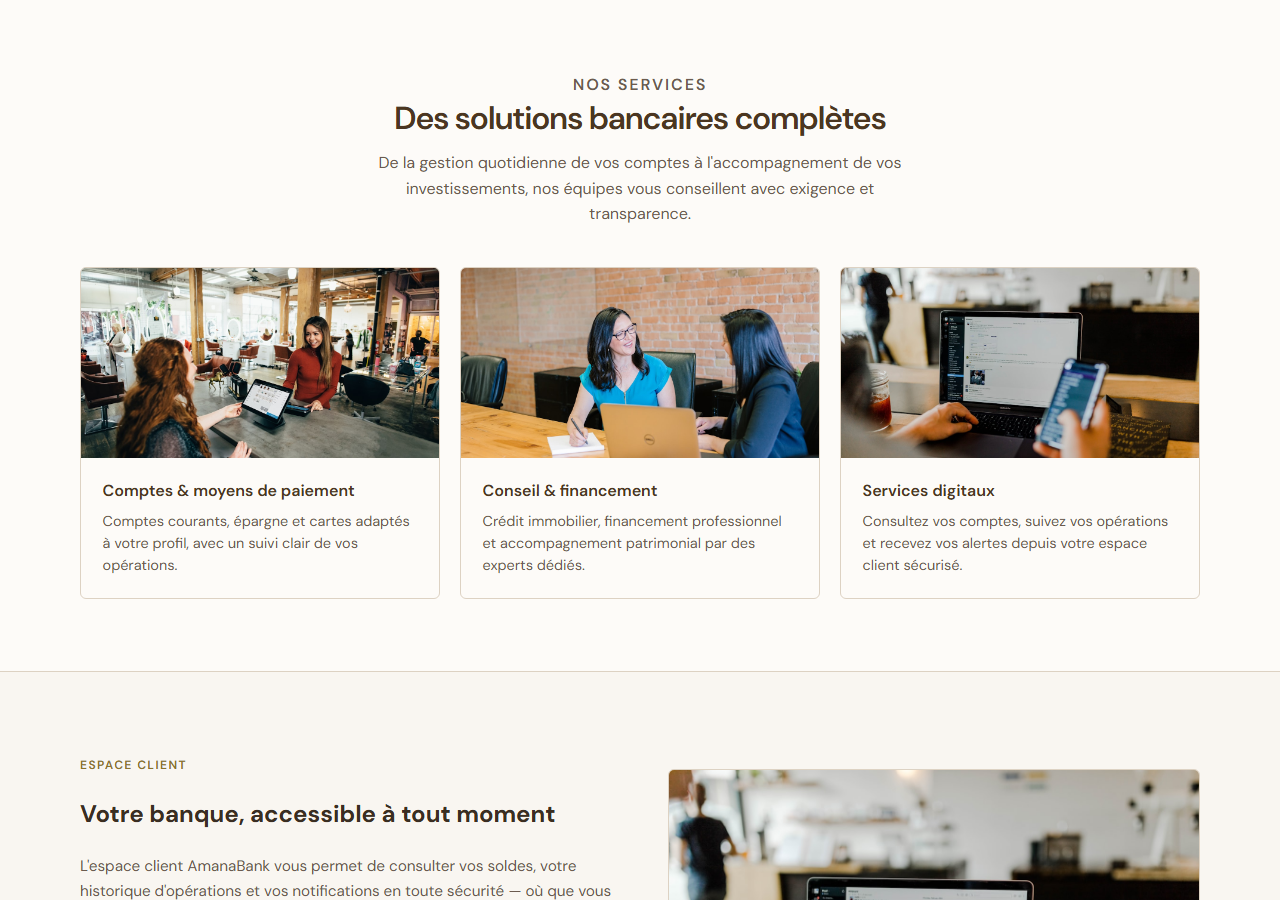
\includegraphics[width=\textwidth]{landing-services.png}%
    }{%
        \fbox{\parbox{0.9\textwidth}{\centering\vspace{2cm}
        \textit{[Capture optionnelle : \texttt{landing-services.png} — grille des services]}
        \vspace{2cm}}}%
    }
    \caption{Page d'accueil — présentation des services et de l'espace client digital}
    \label{fig:landing-services}
\end{figure}

\subsection{Page de connexion}

L'écran de connexion (\texttt{/login}) est le \textbf{point d'entrée unique} pour tous les utilisateurs. Un même formulaire accepte :
\begin{itemize}[leftmargin=*]
    \item le \textbf{personnel} (admin, agent, chef d'agence) via son nom d'utilisateur ;
    \item le \textbf{client} via son CIN ou son numéro client.
\end{itemize}

L'interface comporte le logo AmanaBank centré, des champs avec icônes Bootstrap, un bouton de connexion doré et deux encadrés d'aide rappelant les identifiants de démonstration (ex.\ CIN \texttt{MB654321} pour le client \textbf{Moncef Bensouda}). Un lien «\,Retour à l'accueil\,» permet de revenir à la landing sans utiliser le bouton précédent du navigateur.

\begin{figure}[H]
    \centering
    \IfFileExists{images/login.png}{%
        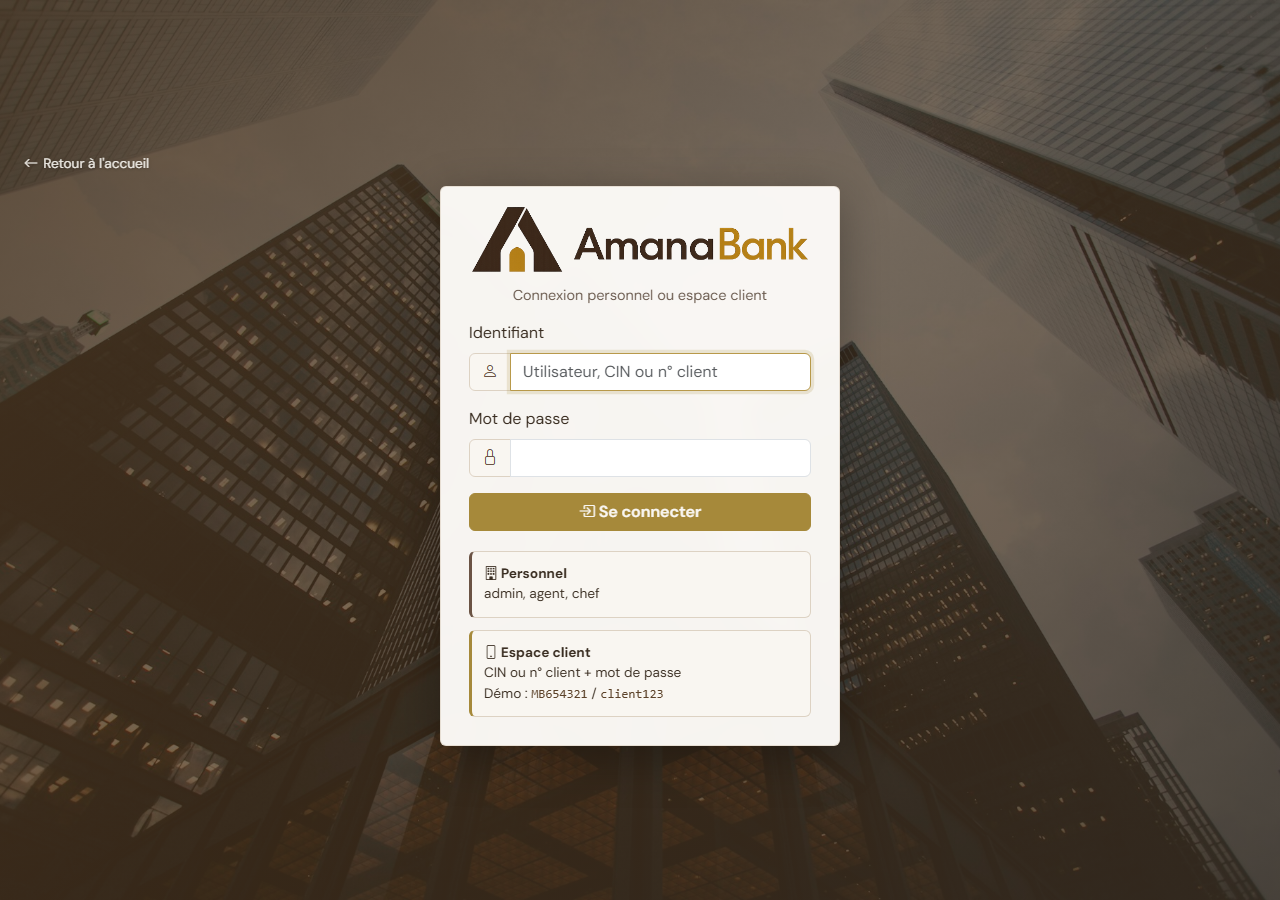
\includegraphics[width=0.75\textwidth]{login.png}%
    }{%
        \fbox{\parbox{0.75\textwidth}{\centering\vspace{2cm}
        \textit{[Capture : \texttt{login.png}]}
        \vspace{2cm}}}%
    }
    \caption{Connexion unifiée — personnel et espace client}
    \label{fig:login}
\end{figure}

\section{Espace agence — personnel}

\subsection{Layout et navigation}

Une fois authentifié, le personnel accède à un \textbf{layout à sidebar} (\texttt{layout/main.html}). La barre latérale marron regroupe les modules métier ; l'élément actif est mis en surbrillance dorée. Le pied de sidebar affiche le nom et le rôle de l'utilisateur connecté, ainsi qu'un bouton de déconnexion.

Le menu s'adapte au \textbf{rôle} :
\begin{itemize}[leftmargin=*]
    \item \textbf{Agent} : clients, comptes, opérations, historique, chéquiers ;
    \item \textbf{Chef d'agence} : mêmes modules + notifications et journal d'audit ;
    \item \textbf{Administrateur} : ajout de la gestion des utilisateurs internes.
\end{itemize}

\subsection{Tableau de bord}

Le tableau de bord (\texttt{/dashboard}) est la \textbf{page d'atterrissage} après connexion. Il synthétise l'activité de l'agence en quatre indicateurs :

\begin{table}[H]
    \centering
    \caption{Indicateurs du tableau de bord agence}
    \label{tab:kpi-agence}
    \small
    \begin{tabular}{@{}lp{8cm}@{}}
        \toprule
        \rowcolor{AmanaBrown}\color{white}
        \textbf{Indicateur} & \textbf{Description et action associée} \\
        \midrule\color{AmanaText}
        Clients actifs & Nombre de clients au statut actif — lien vers la gestion clients \\
        Comptes actifs & Comptes ouverts et non clôturés — lien vers la liste des comptes \\
        Opérations aujourd'hui & Nombre de transactions du jour — lien vers les opérations \\
        Volume du jour & Montant total des opérations du jour — lien vers l'historique \\
        \bottomrule
    \end{tabular}
\end{table}

Des \textbf{alertes métier} apparaissent lorsque des commandes de chéquier sont en attente ou en cours de traitement ; chaque alerte est cliquable et filtre directement la liste correspondante.

En dessous, un tableau récapitule les \textbf{10 dernières opérations} avec accès immédiat au reçu de chaque transaction.

\begin{figure}[H]
    \centering
    \IfFileExists{images/dashboard-agent.png}{%
        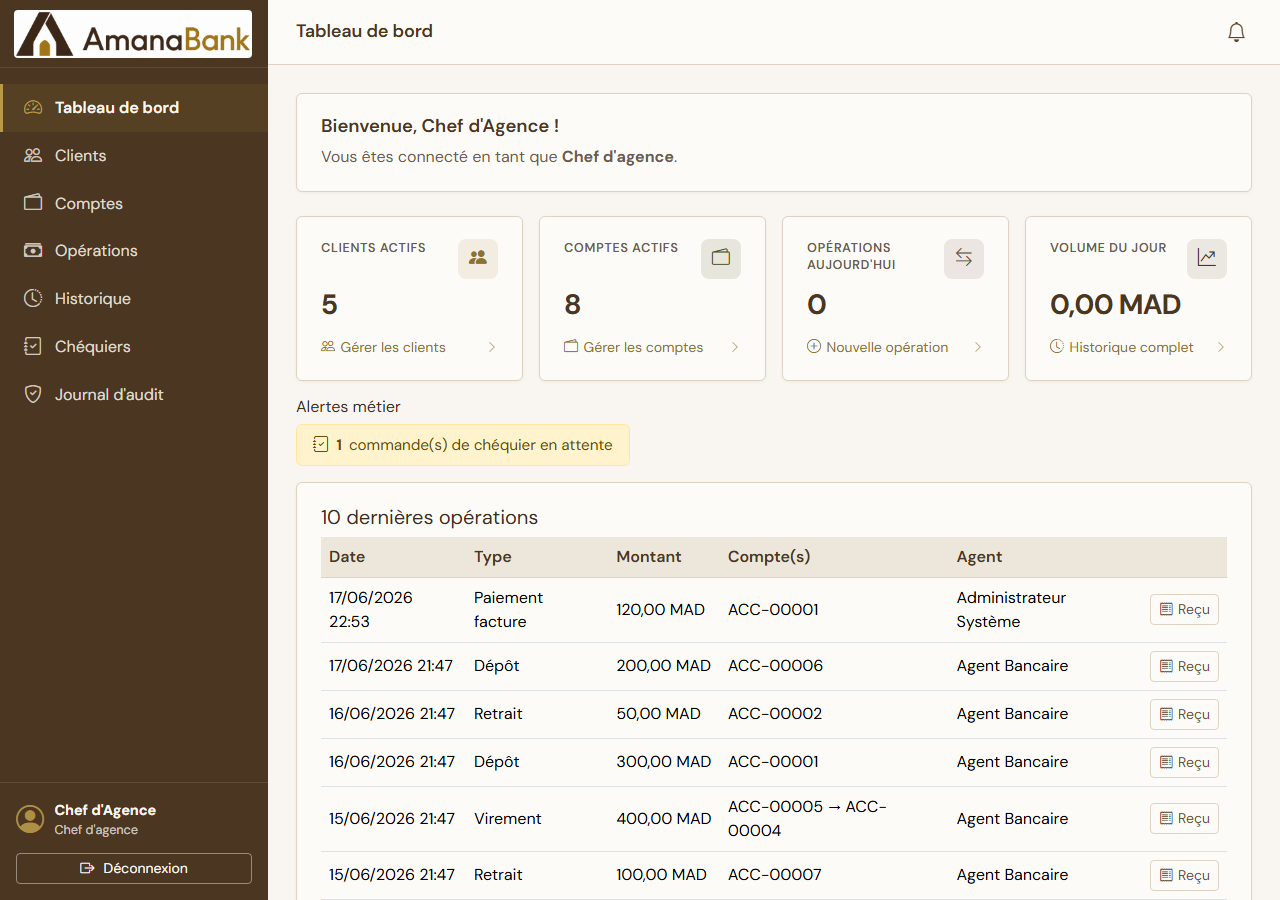
\includegraphics[width=\textwidth]{dashboard-agent.png}%
    }{%
        \fbox{\parbox{0.9\textwidth}{\centering\vspace{2cm}
        \textit{[Capture chef : \texttt{dashboard-agent.png}]}
        \vspace{2cm}}}%
    }
    \caption{Tableau de bord agence — cartes KPI, alertes chéquier et opérations récentes}
    \label{fig:dashboard}
\end{figure}

\subsection{Gestion des clients}

L'écran de liste clients permet la \textbf{recherche}, la création et la consultation des fiches. Chaque fiche regroupe les informations d'identité, le statut (actif, suspendu, fermé) et la liste des comptes associés.

\begin{figure}[H]
    \centering
    \IfFileExists{images/clients-liste.png}{%
        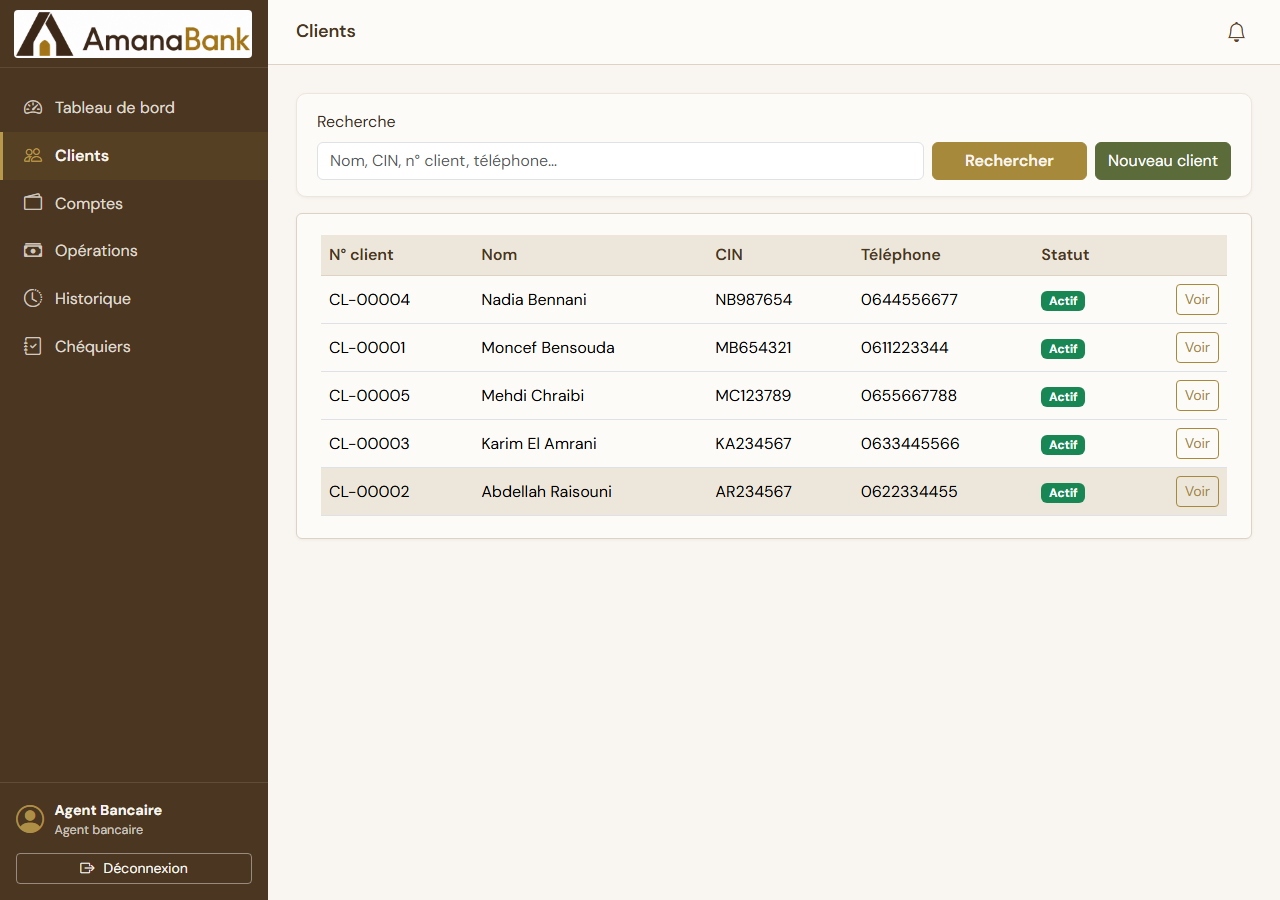
\includegraphics[width=\textwidth]{clients-liste.png}%
    }{%
        \fbox{\parbox{0.9\textwidth}{\centering\vspace{2cm}
        \textit{[Capture : \texttt{clients-liste.png}]}
        \vspace{2cm}}}%
    }
    \caption{Liste et recherche des clients}
    \label{fig:clients}
\end{figure}

\subsection{Comptes bancaires}

La fiche compte affiche le numéro, le type (courant, épargne, professionnel), le solde, le statut et les actions disponibles (blocage, clôture, relevé). La figure~\ref{fig:compte} illustre le compte courant de \textbf{Moncef Bensouda} (\texttt{ACC-00001}), client le plus aisé du jeu de démonstration.

\begin{figure}[H]
    \centering
    \IfFileExists{images/compte-detail.png}{%
        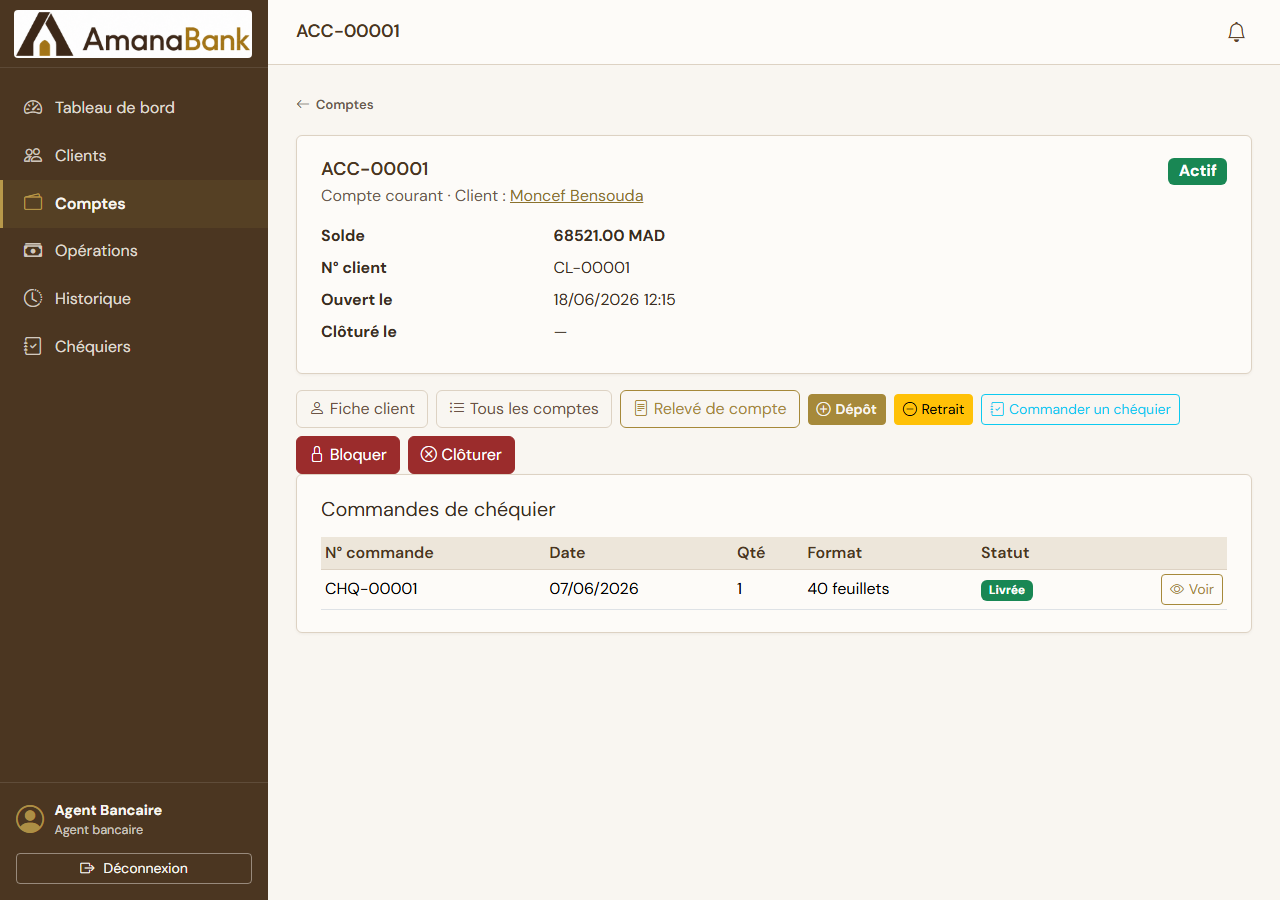
\includegraphics[width=\textwidth]{compte-detail.png}%
    }{%
        \fbox{\parbox{0.9\textwidth}{\centering\vspace{2cm}
        \textit{[Capture : \texttt{compte-detail.png}]}
        \vspace{2cm}}}%
    }
    \caption{Fiche détail — compte courant Moncef Bensouda (\texttt{ACC-00001})}
    \label{fig:compte}
\end{figure}

\subsection{Opérations financières}

Le module opérations regroupe quatre types d'actions, chacune sur un formulaire dédié avec validation côté serveur (montants positifs, solde suffisant, comptes actifs) :

\begin{itemize}[leftmargin=*]
    \item \textbf{Dépôt} — crédit d'un compte ;
    \item \textbf{Retrait} — débit avec contrôle de solde ;
    \item \textbf{Virement} — transfert entre deux comptes ;
    \item \textbf{Paiement de facture} — débit et enregistrement du fournisseur (LYDEC, ONEE, IAM…).
\end{itemize}

\begin{figure}[H]
    \centering
    \IfFileExists{images/operations-depot.png}{%
        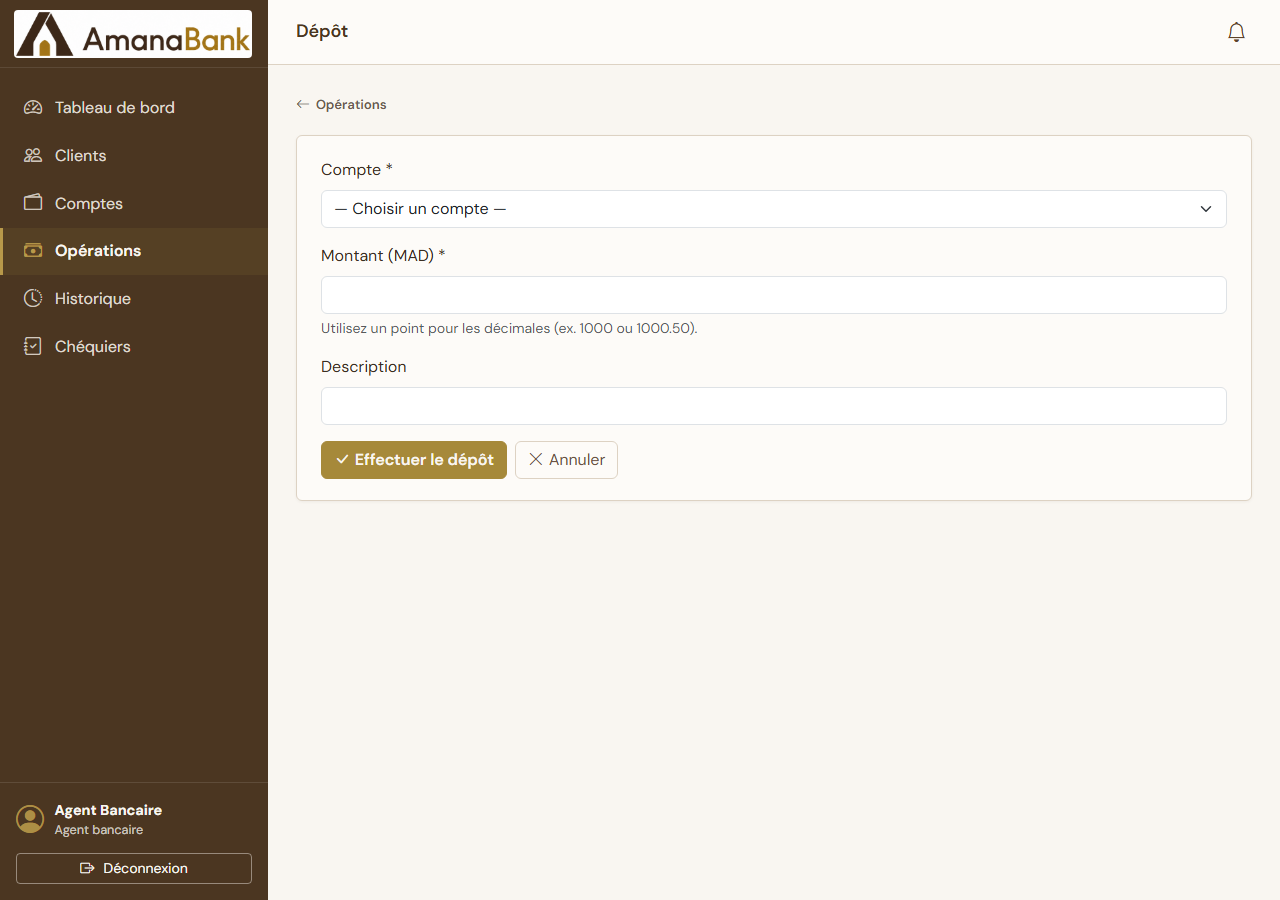
\includegraphics[width=0.85\textwidth]{operations-depot.png}%
    }{%
        \fbox{\parbox{0.85\textwidth}{\centering\vspace{2cm}
        \textit{[Capture : \texttt{operations-depot.png}]}
        \vspace{2cm}}}%
    }
    \caption{Formulaire de dépôt sur compte client}
    \label{fig:depot}
\end{figure}

\begin{figure}[H]
    \centering
    \IfFileExists{images/paiement-facture.png}{%
        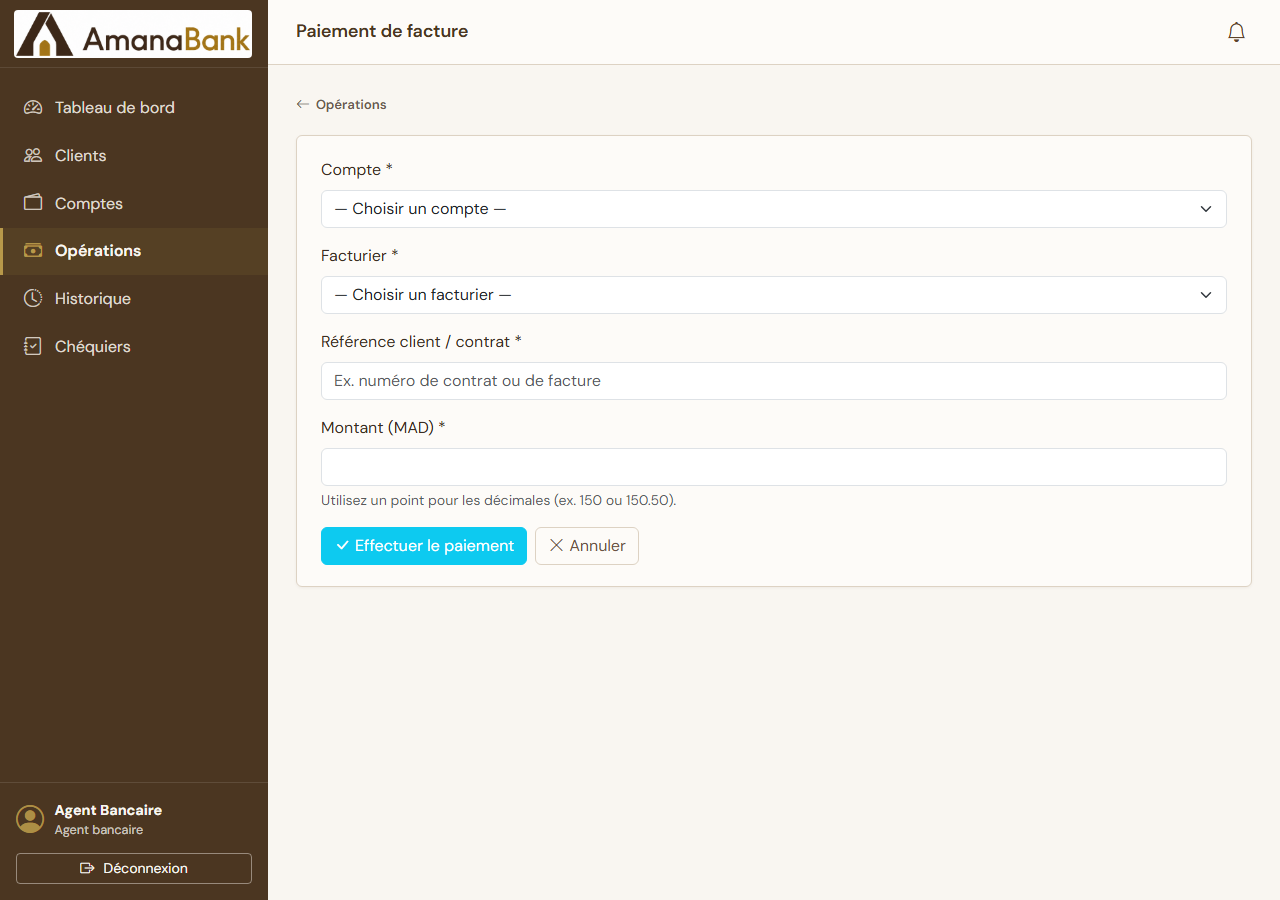
\includegraphics[width=0.85\textwidth]{paiement-facture.png}%
    }{%
        \fbox{\parbox{0.85\textwidth}{\centering\vspace{2cm}
        \textit{[Capture : \texttt{paiement-facture.png}]}
        \vspace{2cm}}}%
    }
    \caption{Paiement de facture — sélection du fournisseur et du compte}
    \label{fig:facture}
\end{figure}

\subsection{Historique et reçu PDF}

Chaque opération génère une entrée dans l'historique. La page de reçu présente le détail de la transaction et propose le \textbf{téléchargement PDF} via OpenPDF, avec un nom de fichier normalisé.

\begin{figure}[H]
    \centering
    \IfFileExists{images/recu-pdf.png}{%
        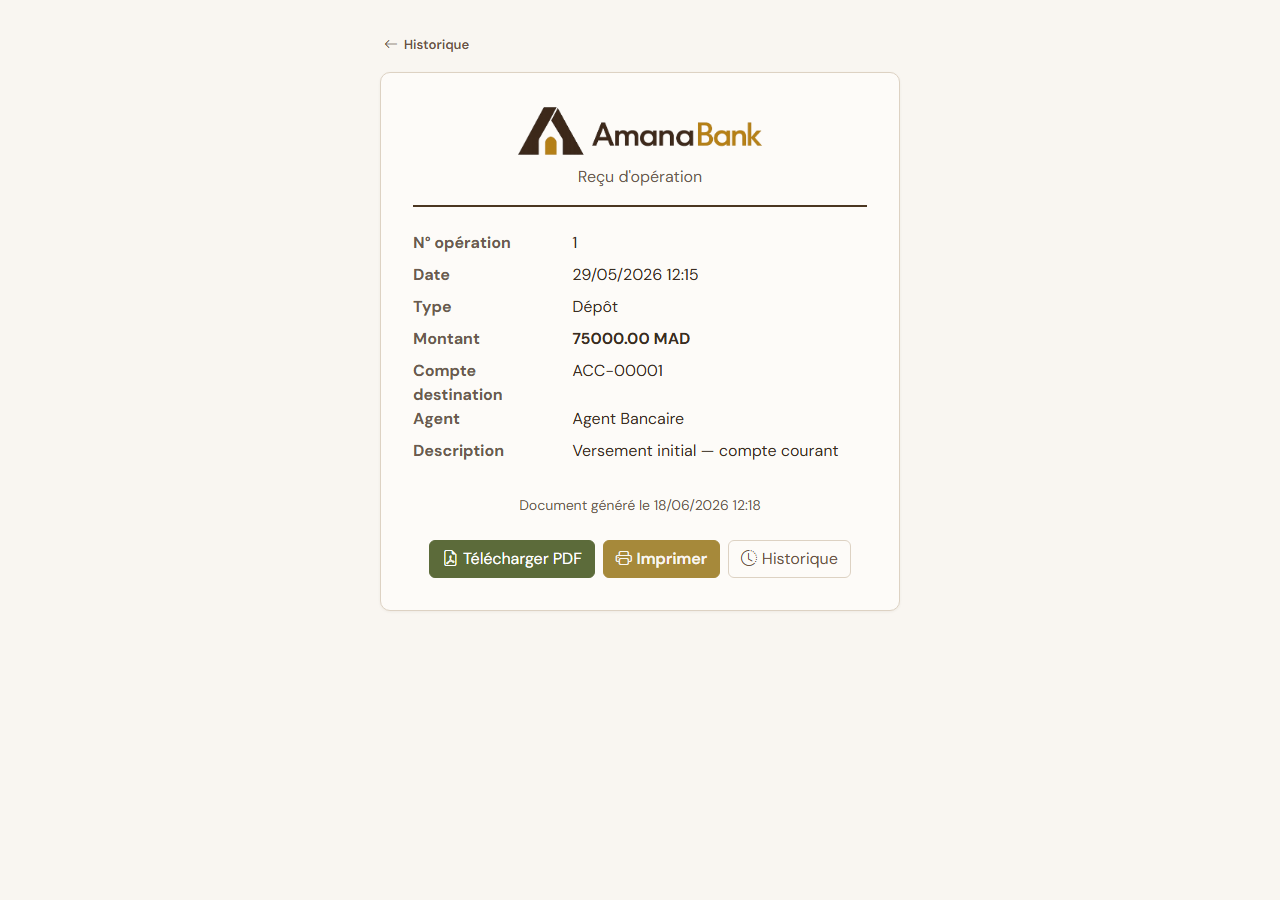
\includegraphics[width=\textwidth]{recu-pdf.png}%
    }{%
        \fbox{\parbox{0.9\textwidth}{\centering\vspace{2cm}
        \textit{[Capture : \texttt{recu-pdf.png}]}
        \vspace{2cm}}}%
    }
    \caption{Reçu d'opération avec bouton de téléchargement PDF}
    \label{fig:recu}
\end{figure}

\subsection{Commandes de chéquier et notifications}

Les commandes de chéquier suivent un \textbf{workflow} sans impact sur le solde : demande, traitement, livraison. Le chef d'agence reçoit des notifications et peut consulter le centre dédié via la cloche en en-tête.

\begin{figure}[H]
    \centering
    \IfFileExists{images/chequier-liste.png}{%
        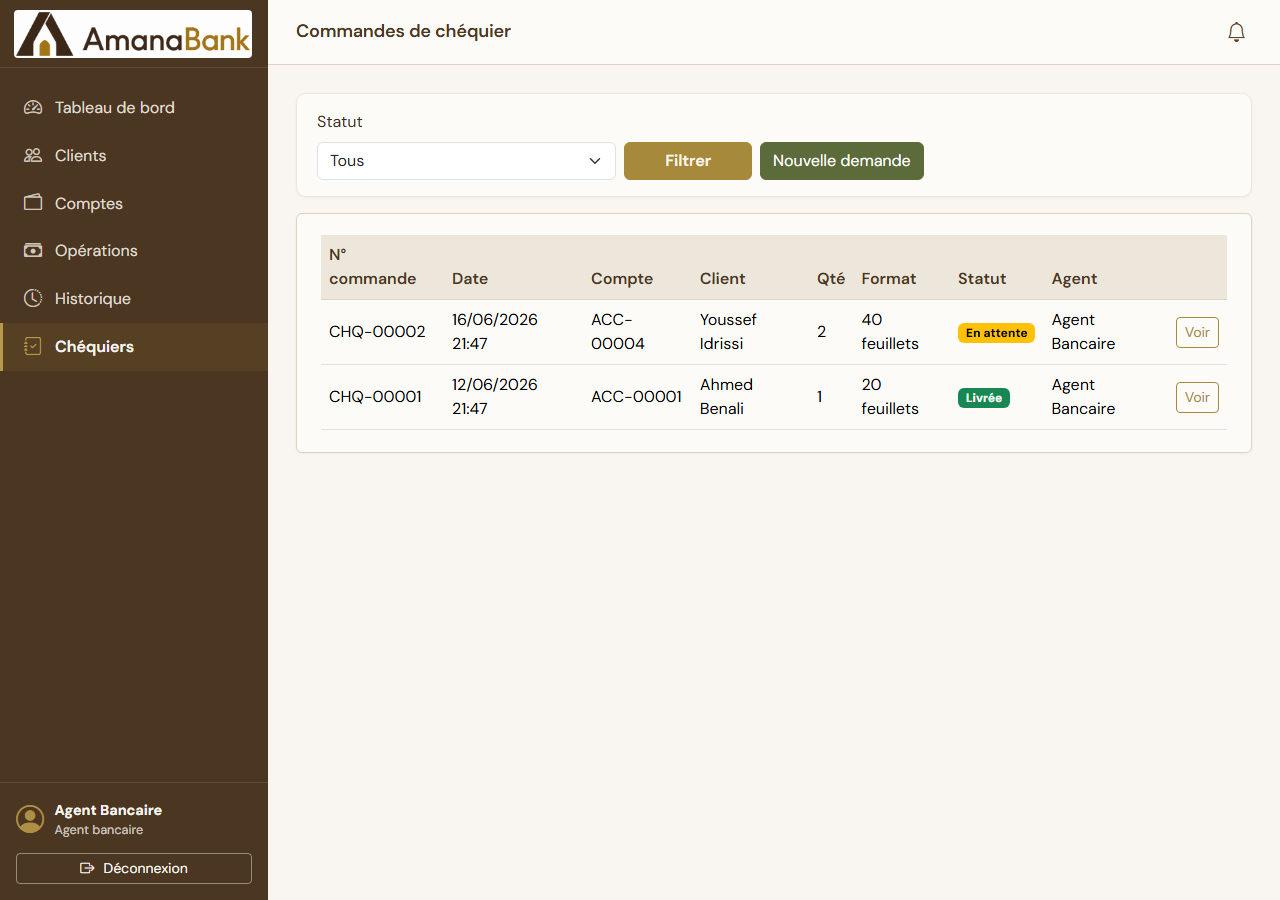
\includegraphics[width=\textwidth]{chequier-liste.png}%
    }{%
        \fbox{\parbox{0.9\textwidth}{\centering\vspace{2cm}
        \textit{[Capture : \texttt{chequier-liste.png}]}
        \vspace{2cm}}}%
    }
    \caption{Suivi des commandes de chéquier par statut}
    \label{fig:chequier}
\end{figure}

\begin{figure}[H]
    \centering
    \IfFileExists{images/notifications.png}{%
        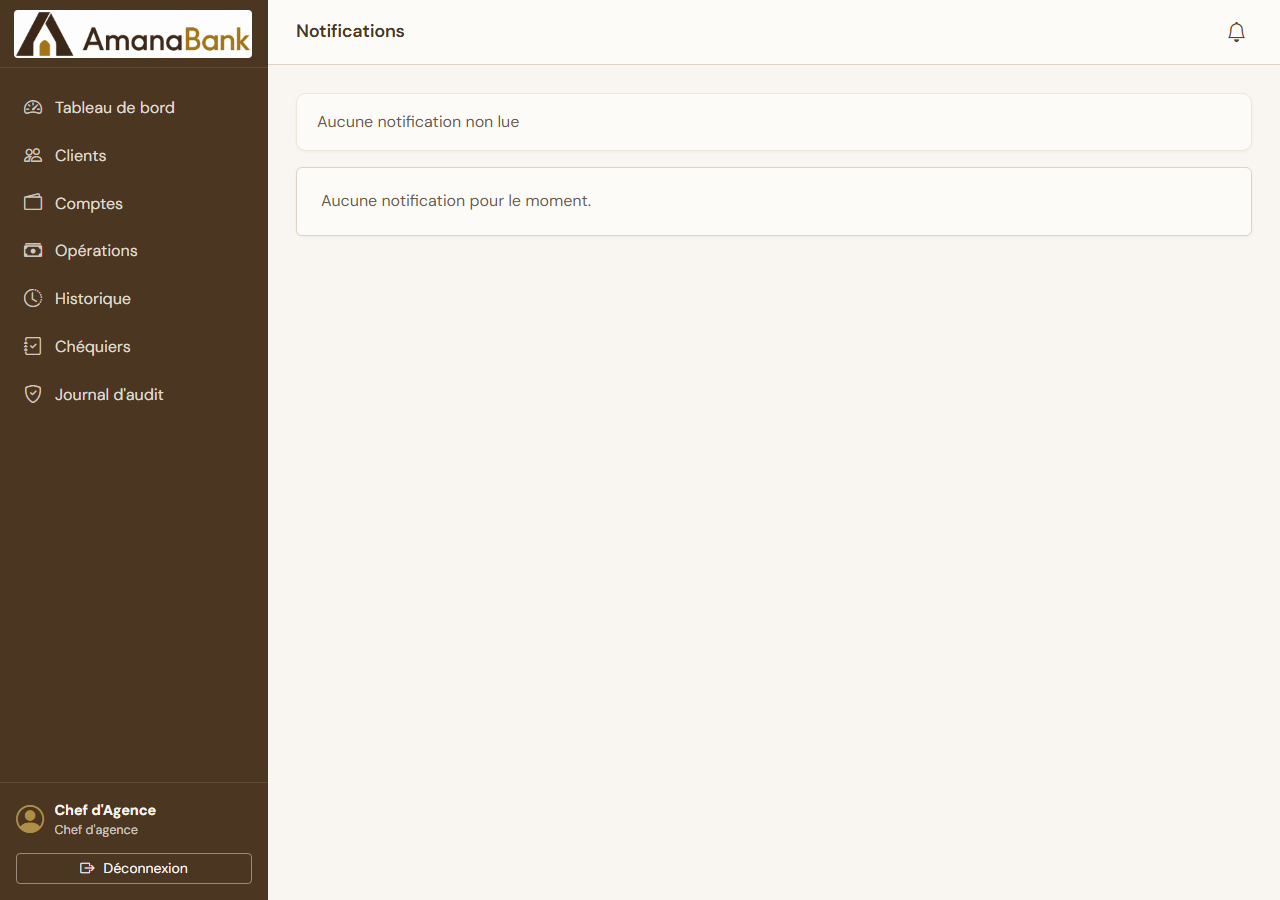
\includegraphics[width=\textwidth]{notifications.png}%
    }{%
        \fbox{\parbox{0.9\textwidth}{\centering\vspace{2cm}
        \textit{[Capture : \texttt{notifications.png}]}
        \vspace{2cm}}}%
    }
    \caption{Centre de notifications — chef d'agence}
    \label{fig:notifications}
\end{figure}

\subsection{Administration}

L'administrateur gère les comptes du personnel (création, modification, réinitialisation de mot de passe). Le journal d'audit, accessible au chef et à l'admin, recense les actions sensibles pour la traçabilité.

\begin{figure}[H]
    \centering
    \IfFileExists{images/admin-users.png}{%
        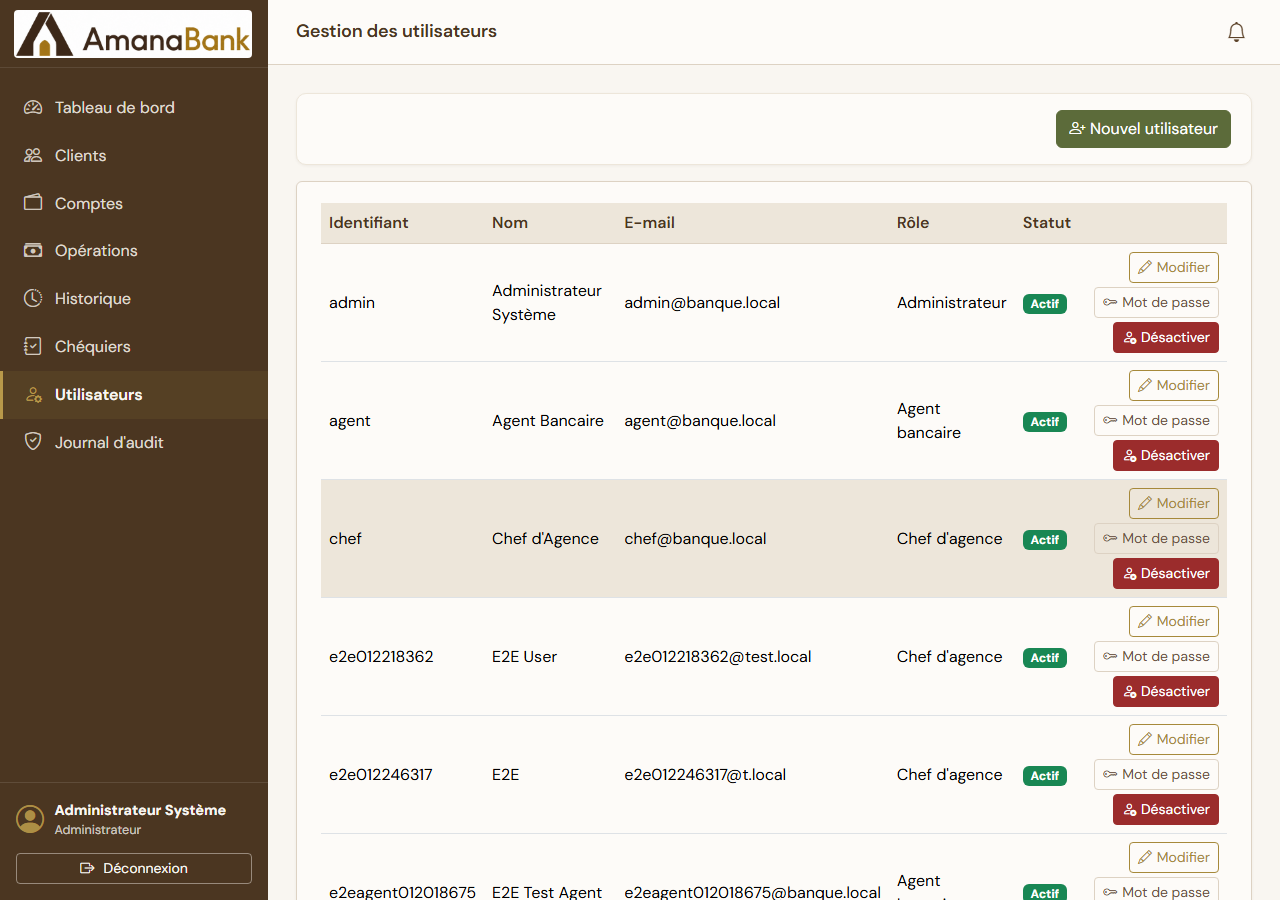
\includegraphics[width=\textwidth]{admin-users.png}%
    }{%
        \fbox{\parbox{0.9\textwidth}{\centering\vspace{2cm}
        \textit{[Capture : \texttt{admin-users.png}]}
        \vspace{2cm}}}%
    }
    \caption{Gestion des utilisateurs internes}
    \label{fig:admin}
\end{figure}

\section{Espace client (portail)}

\subsection{Présentation générale}

Le portail client (\texttt{/portal/**}) offre une \textbf{consultation en lecture seule} : soldes, historique, notifications et suivi des chéquiers. Il reprend le même layout à sidebar que l'espace agence, avec un badge «\,Espace client\,» et un menu adapté.

\subsection{Tableau de bord client}

Le dashboard client synthétise la situation du titulaire :

\begin{itemize}[leftmargin=*]
    \item \textbf{Solde total} — somme des comptes actifs ;
    \item \textbf{Nombre de comptes} — accès rapide au détail ;
    \item \textbf{Notifications non lues} — alertes sur les opérations effectuées en agence ;
    \item \textbf{Chéquiers en cours} — commandes en attente ou en traitement.
\end{itemize}

Des cartes individuelles affichent chaque compte (type, numéro, solde, badge de statut). La figure~\ref{fig:portal} montre l'espace de \textbf{Moncef Bensouda} (CIN \texttt{MB654321}), dont le solde total dépasse 600\,000~MAD sur trois comptes. Le tableau des \textbf{5 dernières opérations} permet de télécharger les reçus PDF.

\begin{figure}[H]
    \centering
    \IfFileExists{images/portal-dashboard.png}{%
        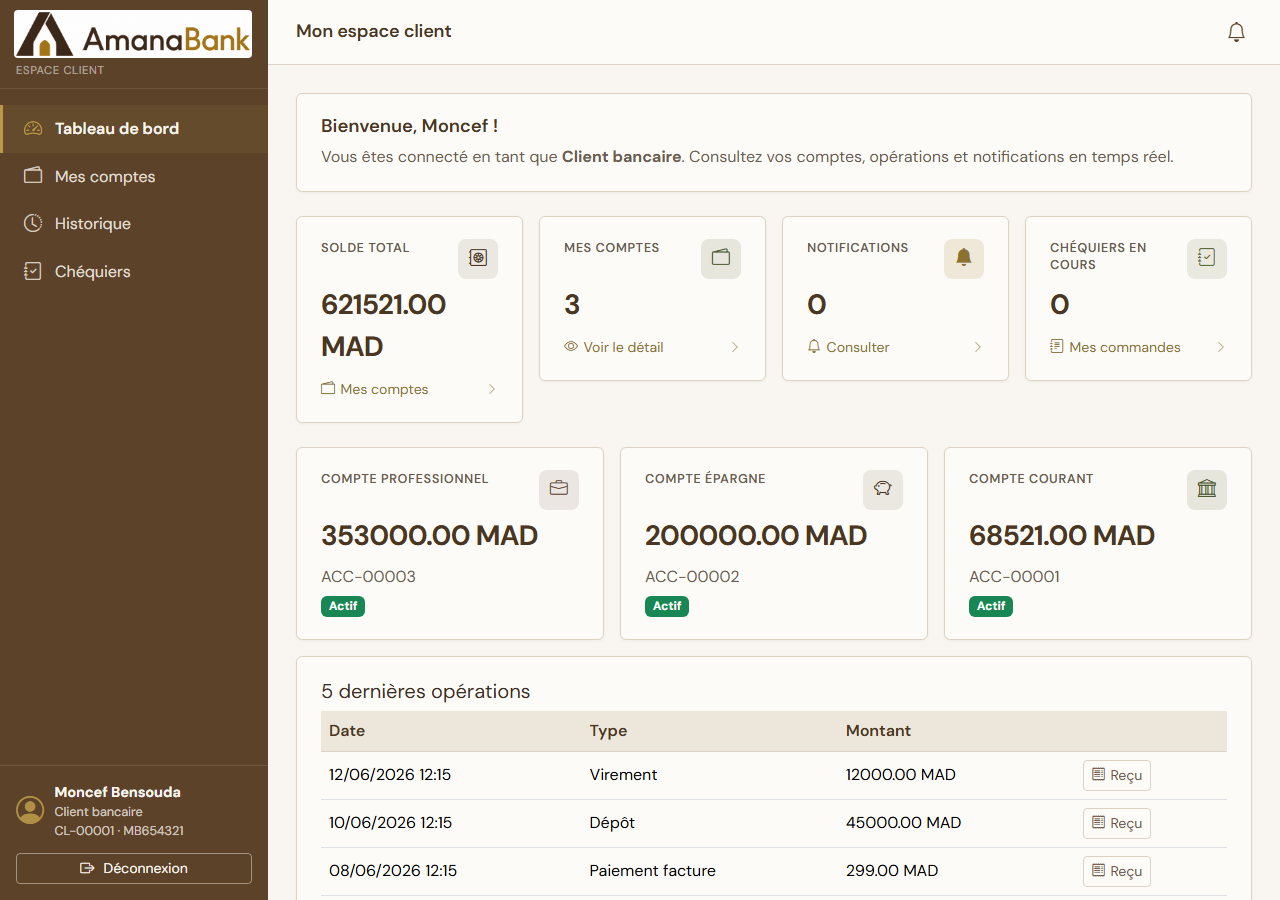
\includegraphics[width=\textwidth]{portal-dashboard.png}%
    }{%
        \fbox{\parbox{0.9\textwidth}{\centering\vspace{2cm}
        \textit{[Capture : \texttt{portal-dashboard.png}]}
        \vspace{2cm}}}%
    }
    \caption{Tableau de bord espace client — KPI, comptes et historique récent}
    \label{fig:portal}
\end{figure}

\begin{figure}[H]
    \centering
    \IfFileExists{images/portal-notifications.png}{%
        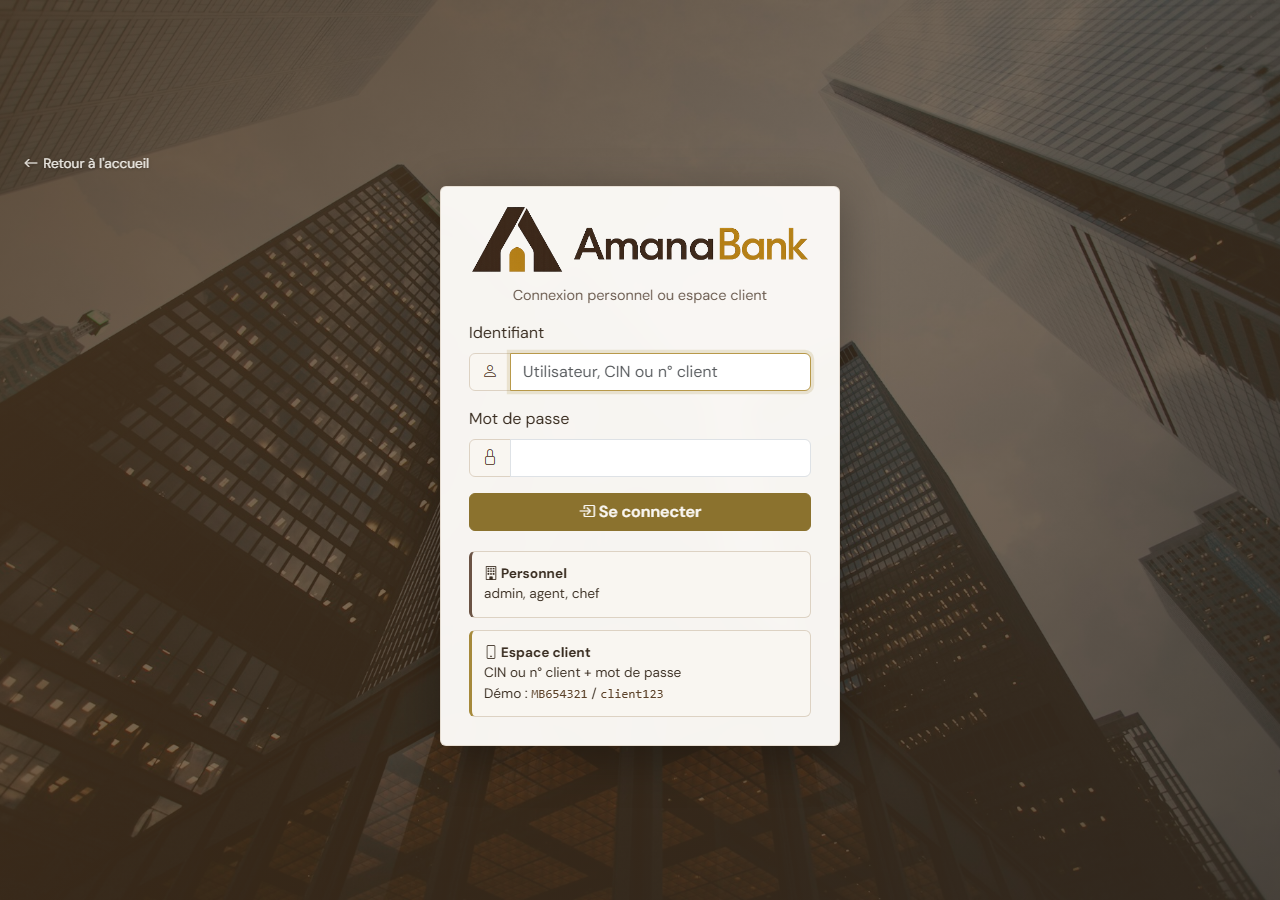
\includegraphics[width=\textwidth]{portal-notifications.png}%
    }{%
        \fbox{\parbox{0.9\textwidth}{\centering\vspace{2cm}
        \textit{[Capture : \texttt{portal-notifications.png}]}
        \vspace{2cm}}}%
    }
    \caption{Notifications client — opérations et mises à jour chéquier}
    \label{fig:portal-notif}
\end{figure}

\section{Conclusion}

Ce chapitre a présenté les interfaces réalisées pour \nomapplication, de la vitrine publique aux espaces connectés. Les choix de conception — charte AmanaBank unifiée, cartes KPI informatives, navigation par rôle et formulaire de connexion unique — visent une expérience \textbf{claire, professionnelle et cohérente} pour chaque type d'utilisateur.

L'ensemble des écrans métier (clients, comptes, opérations, reporting) s'appuie sur les mêmes composants visuels, ce qui facilite la prise en main par le personnel et renforce l'image de marque auprès des clients.

\chapter*{Conclusion générale}
\addcontentsline{toc}{chapter}{Conclusion générale}

\section*{Conclusion}

La réalisation de ce projet de fin d'année, intitulé \textbf{\nomapplication}, nous a permis de mener un développement web complet, de la conception UML jusqu'à une application fonctionnelle et testée. Destinée à la gestion d'une agence bancaire, cette plateforme répond aux exigences du cahier des charges et intègre des extensions métier : paiement de factures, commande de chéquier, notifications et portail client.

\section*{Bilan}

\begin{itemize}[leftmargin=*]
    \item \textbf{Conception} : diagrammes UML complets (cas d'utilisation, classes, séquences, activité, MCD/MLD).
    \item \textbf{Implémentation} : 11 migrations Flyway, 9 entités JPA, architecture en couches Spring Boot.
    \item \textbf{Fonctionnalités} : gestion clients/comptes, opérations financières contrôlées, admin, audit, reporting, reçus PDF.
    \item \textbf{Extensions} : factures, chéquier, notifications bidirectionnelles, portail client lecture seule.
    \item \textbf{Qualité} : 80 tests d'intégration, seed de démo modulaire, documentation technique complète.
    \item \textbf{Interface} : refonte graphique complète — landing marketing, login unifié, dashboards KPI et charte AmanaBank (marron/beige/or, DM Sans).
\end{itemize}

Les objectifs fixés en introduction ont été atteints : centralisation des données, respect des règles métier, traçabilité et expérience utilisateur adaptée à chaque rôle.

\section*{Difficultés rencontrées}

\begin{itemize}[leftmargin=*]
    \item \textbf{Configuration PostgreSQL} : conflit de ports locaux (5432 occupé) — résolu en utilisant le port 5433.
    \item \textbf{Cohérence transactionnelle} : gestion des soldes avec verrouillage optimiste (\texttt{@Version}) et \texttt{@Transactional}.
    \item \textbf{Authentification dual} : un seul formulaire de login pour personnel et clients — résolu via \texttt{UserDetailsServiceImpl} composite.
    \item \textbf{Portail sur base existante} : synchronisation des accès client via \texttt{DemoPortalSync} au démarrage.
    \item \textbf{Workflow chéquier} : distinguer service administratif (sans mouvement financier) des transactions.
\end{itemize}

\section*{Perspectives d'évolution}

\begin{itemize}[leftmargin=*]
    \item Export PDF des \textbf{relevés de compte} (reçus déjà en PDF).
    \item API REST documentée (Swagger) pour intégrations futures.
    \item Pipeline CI/CD (GitHub Actions) et déploiement conteneurisé.
    \item Enrichissement du portail client (demandes en ligne, messagerie).
    \item Authentification à deux facteurs (2FA) pour le personnel.
    \item Tableau de bord analytique avancé (graphiques, exports Excel).
\end{itemize}

\vspace{0.5cm}
En conclusion, \nomapplication\ constitue une solution concrète et défendable pour la digitalisation d'une agence bancaire. Ce PFA nous a permis de consolider nos compétences en conception orientée objet, développement Java/Spring et travail en binôme, et constitue une base solide pour nos futurs projets professionnels.

\vspace{1cm}
\begin{flushright}
    \etudianteun\\
    \etudiantedeux
\end{flushright}

\begin{thebibliography}{99}
\addcontentsline{toc}{chapter}{Bibliographie}

\bibitem{spring-boot}
Spring Boot Documentation, VMware / Broadcom.
\url{https://docs.spring.io/spring-boot/docs/current/reference/html/} (consulté en 2026).

\bibitem{spring-security}
Spring Security Reference Documentation.
\url{https://docs.spring.io/spring-security/reference/} (consulté en 2026).

\bibitem{spring-data-jpa}
Spring Data JPA Documentation.
\url{https://docs.spring.io/spring-data/jpa/docs/current/reference/html/} (consulté en 2026).

\bibitem{thymeleaf}
Thymeleaf Documentation.
\url{https://www.thymeleaf.org/documentation.html} (consulté en 2026).

\bibitem{postgresql}
PostgreSQL Documentation, Version 18.
\url{https://www.postgresql.org/docs/} (consulté en 2026).

\bibitem{flyway}
Flyway Documentation, Redgate.
\url{https://documentation.red-gate.com/fd} (consulté en 2026).

\bibitem{bootstrap}
Bootstrap Documentation, Version 5.3.
\url{https://getbootstrap.com/docs/5.3/} (consulté en 2026).

\bibitem{openpdf}
OpenPDF — Libre PDF Library.
\url{https://github.com/LibrePDF/OpenPDF} (consulté en 2026).

\bibitem{uml}
OMG — Unified Modeling Language Specification.
\url{https://www.omg.org/spec/UML/} (consulté en 2026).

\bibitem{plantuml}
PlantUML — Open-source tool for UML diagrams.
\url{https://plantuml.com/} (consulté en 2026).

\bibitem{cahier}
Cahier des charges PFA — Système de gestion d'agence bancaire.
\texttt{documentation/cahier-charge-PFA.pdf}, projet \nomapplication.

\bibitem{gantt}
GanttProject — Project scheduling application.
\url{https://www.ganttproject.biz/} (consulté en 2026).

\end{thebibliography}

\end{document}
